\documentclass{ieeeaccess}
%% Paper 2: "Can experience-sampling EEG identify a state-space model of meditation
%% dynamics? A preregistered test on two open datasets" (IEEE Access template).
%% This is the master file only; the content lives in the child files:
%%   preamble.tex            packages, macros, graphics path
%%   frontmatter.tex         title, authors, abstract, index terms
%%   sections/1_introduction.tex, 2_literature_review, 3_theoretical_framework (BQI),
%%   4_methodology, 5_results, 6_discussion (incl. limitations), 7_conclusion, 8_appendices
%%   references.bib          BibTeX database (IEEEtran.bst, citation order)
%%   biography.tex           author biography
%% Figures are read from ../outputs/paper/{eeg,realdata,osf3uszv}/.
%% The original sample of the template is kept as access_sample_original.tex.
%% Compile from this folder:
%%   pdflatex access && bibtex access && pdflatex access && pdflatex access
%% Packages, bold-math set-up of the IEEE Access template, graphics path and macros.
%% Input by access.tex before \begin{document}.
\usepackage{cite}
\usepackage{amsmath,amssymb,amsfonts}
\usepackage{graphicx}
\usepackage{textcomp}
\usepackage{booktabs}
\usepackage{url}
\usepackage{bm}
\makeatletter
\AtBeginDocument{\DeclareMathVersion{bold}
\SetSymbolFont{operators}{bold}{T1}{times}{b}{n}
\SetSymbolFont{NewLetters}{bold}{T1}{times}{b}{it}
\SetMathAlphabet{\mathrm}{bold}{T1}{times}{b}{n}
\SetMathAlphabet{\mathit}{bold}{T1}{times}{b}{it}
\SetMathAlphabet{\mathbf}{bold}{T1}{times}{b}{n}
\SetMathAlphabet{\mathtt}{bold}{OT1}{pcr}{b}{n}
\SetSymbolFont{symbols}{bold}{OMS}{cmsy}{b}{n}
\renewcommand\boldmath{\@nomath\boldmath\mathversion{bold}}}
\makeatother

\graphicspath{{../outputs/paper/eeg/}{../outputs/paper/realdata/}{../outputs/paper/osf3uszv/}}

\newcommand{\kinh}{k_{\mathrm{inh}}}
\newcommand{\kd}{k_{d}}
\newcommand{\sA}{\sigma_{A}}
\newcommand{\sPhi}{\sigma_{\Phi}}
\newcommand{\rA}{r_{A}}
\newcommand{\rPhi}{r_{\Phi}}
\newcommand{\rQ}{r_{Q}}
\newcommand{\CRB}{\mathrm{CRB}}
\newcommand{\RMSE}{\mathrm{RMSE}}
\newcommand{\QoC}{\mathrm{QoC}}
\newcommand{\dd}{\,\mathrm{d}}
\newcommand{\thetav}{\boldsymbol{\theta}}
\newcommand{\xv}{\mathbf{x}}
\newcommand{\yv}{\mathbf{y}}
\newcommand{\Cov}{\operatorname{Cov}}
\newcommand{\diag}{\operatorname{diag}}
% notation of the BQI paper (D. Q. Vu, paper/bqi_paper.pdf)
\newcommand{\ADMN}{A_{\mathrm{DMN}}}
\newcommand{\kint}{k_{\mathrm{int}}}
\newcommand{\kspont}{k_{\mathrm{spont}}}
\newcommand{\Amax}{A_{\max}}
\newcommand{\PCI}{\mathrm{PCI}}
\newcommand{\LZC}{\mathrm{LZC}}
\newcommand{\KL}{\mathrm{KL}}

% Reference [BQI] (D. Q. Vu, paper/bqi_paper.pdf) has no DOI or preprint yet: its entry in the
% reference list is printed in red until it does. Delete this block once the DOI is in references.bib.
\makeatletter
\def\BQI@key{BQI}
\newcommand{\BQI@wrapbibitem}[1]{\normalcolor\BQI@origbibitem{#1}\def\BQI@this{#1}%
  \ifx\BQI@this\BQI@key\color{red}\fi}
\AtBeginDocument{\let\BQI@origbibitem\bibitem\let\bibitem\BQI@wrapbibitem}
\makeatother


\begin{document}
%% Title block, abstract and index terms. Input by access.tex right after \begin{document}.
%% TODO: author list, e-mail and DOI before submission.
\history{Date of publication xxxx 00, 0000, date of current version xxxx 00, 0000.}
\doi{10.1109/ACCESS.2026.0000000}

\title{From Equations to Electrodes: A Preregistered Test of the Brain-as-a-Query-Interface Model of Meditation on Two Open EEG Datasets}
% TODO: confirm the author list and affiliations before submission (same block as the companion paper).
\author{\uppercase{Dung Vu}\authorrefmark{1}}
\address[1]{Phenikaa University, Hanoi 12116, Vietnam (e-mail: [institutional e-mail])}
\tfootnote{This work was carried out at Phenikaa University, Hanoi. All computations were run on personal computers; no external funding was received.}

\markboth
{Vu: From Equations to Electrodes: Testing the BQI Model of Meditation on EEG}
{Vu: From Equations to Electrodes: Testing the BQI Model of Meditation on EEG}

\corresp{Corresponding author: Dung Vu (e-mail: [institutional e-mail]).}

\begin{abstract}
Dynamical models that link default-mode-network activity, information integration and a reported quality of meditation are increasingly proposed, and a design analysis based on the exact Fisher information of a linear-Gaussian state-space model has recently predicted how precisely such a model can be estimated from experience-sampling electroencephalography (EEG). Whether those predictions hold on real recordings had not been tested. We fitted the model to two open experience-sampling EEG datasets from different laboratories, ds001787 (24 practitioners, 40 sessions, 983 self-report probes) and OSF 3uszv (58 participants, 58 sessions, 2,258 probes), under two preregistrations locked with cryptographic hashes and four machine-checked verification gates each. On both datasets the relative error of the default-mode rate constant predicted before the lock was close to the Fisher standard error at the estimate and to the parametric-bootstrap error (9.1, 9.9 and 9.7 percent on ds001787; 6.7, 8.5 and 8.8 percent on OSF 3uszv), whereas the observed-information error of the alpha-power channel exceeded the Fisher value, a signature of misspecification that was absent in data simulated from the fit. Neither EEG proxy improved the out-of-sample prediction of the self-reports over null models on either dataset. The rate constants themselves did not replicate: the default-mode time constant was 0.76 minutes on ds001787 and 7.1 minutes on OSF 3uszv, and a simulation shows that an Ornstein--Uhlenbeck fit returns the dominant time scale of whatever feature it is given. Design analyses of this kind can be trusted for the precision they promise, but not for the meaning of parameters estimated from uncalibrated proxies.
\end{abstract}

\begin{keywords}
Cram\'er--Rao bound, default mode network, EEG, experience sampling, Fisher information, Kalman filter, meditation, model misspecification, preregistration, state-space model.
\end{keywords}

\titlepgskip=-21pt

\maketitle


%% I. Introduction: background, problem, gap, research questions, contributions, organisation. Input by access.tex.
\section{Introduction}
\label{sec:intro}
\PARstart{M}{editation} research has moved from mean differences between meditators and controls towards models of the dynamics of a session: the alternation between focused attention, mind wandering and meta-awareness \cite{Hasenkamp2012,Lutz2008,Christoff2016}, the regulation of the default mode network (DMN) \cite{Raichle2001,Brewer2011,Garrison2015}, and computational accounts in terms of predictive processing \cite{Laukkonen2021,SandvedSmith2021}. The Brain as a Query Interface (BQI) framework of Vu \cite{BQI} writes these dynamics as differential equations that link DMN activity, integrated information $\Phi$ and a reported quality of consciousness (QoC), fits their rates and gains to meta-analytic data, and proposes to steer them with a closed-loop brain--computer interface \cite[Sec.~7.2, 9.3 and 10.1]{BQI}; it is the theoretical foundation of the present study (Section~\ref{sec:theory}). Models of this kind promise quantities that can be estimated from data, such as the rate at which the DMN is suppressed and the weight of each latent state in the report, and they are put forward as the basis of model-based neurofeedback \cite{Sitaram2017}.

Whether these quantities can be estimated from the data that meditation studies actually collect, continuous EEG and a few self-report probes per session, is a separate question. In a companion paper \cite{companion} we replaced the BQI equations by a linear-Gaussian state-space model (M1) and used its exact expected Fisher information to compute how many subjects, how long a session, how frequent a probe and how clean an EEG feature are needed to estimate each parameter to a given precision. That design analysis was validated on simulated data only. No study has yet tested such a design analysis on real recordings, compared the estimates with the values that BQI derived from the literature, or asked whether the estimated parameters transfer from one laboratory to another (Section~\ref{sec:gap}).

These questions are hard to answer cleanly. The EEG features that stand in for the DMN and for $\Phi$ are proxies without a calibrated mapping to the state variables; a third of the recording can be missing; the model may be misspecified in ways that a bound cannot anticipate; and an analysis with many free choices (features, artefact rules, null models, exclusion criteria) can support almost any conclusion after the fact. We therefore preregistered the whole analysis plan for each of two open datasets, locked it with a SHA-256 hash before the EEG was examined \cite{Nosek2018}, organised the pipeline as a sequence of machine-checked gates that refuse to proceed when a prerequisite fails, and report every locked analysis whether or not it supported the predictions.

\subsection{Research Questions}
\begin{enumerate}
  \item[RQ1] \emph{Precision.} On a real experience-sampling design, with irregular probes, missing epochs and artefact rejection, is the relative error of the hardest parameter, the DMN rate constant $\kinh$, close to the Cram\'er--Rao bound (CRB) computed from the real probe schedules before the EEG is seen?
  \item[RQ2] \emph{Prediction.} Does a model that is identifiable in principle, fitted to continuous EEG and sparse self-reports, predict the reports out of sample better than models that ignore the dynamics?
  \item[RQ3] \emph{Agreement with BQI.} Do the estimated rate constants, coupling and gains agree with the values that BQI fitted to meta-analytic data?
  \item[RQ4] \emph{Replication.} Do the estimated parameters mean the same thing across recordings made in different laboratories with different amplifiers, montages, probe schedules and rating scales?
\end{enumerate}

\subsection{Contributions}
\begin{enumerate}
  \item The first test, to our knowledge, of a Fisher-information design analysis for a dynamical model of meditation against real experience-sampling EEG, on two independent open datasets, ds001787 \cite{Brandmeyer2018,Delorme2024ds} and OSF 3uszv \cite{RodriguezLarios2021}, under two locked preregistrations and eight verification gates.
  \item A reporting scheme of three error numbers, the CRB computed before the lock, the Fisher standard error at the estimate, and the parametric-bootstrap error, together with the observed-information error and a comparison with data simulated from the fit. On both datasets the first three agree for the DMN rate constant, and the fourth exposes a misspecification of the alpha-power channel \cite{White1982}.
  \item A preregistered out-of-sample test of the model against three null models, which shows that neither EEG proxy carries information about the reports beyond the reports' own serial dependence, on either dataset.
  \item A comparison of the estimates with the parameter values of BQI, and preregistered replication checks between the datasets, which show that the rate constants and the group difference between experienced and novice meditators do not transfer, together with a simulation that explains why: an Ornstein--Uhlenbeck fit returns the dominant time scale of the feature it is given.
  \item A fully reproducible pipeline (one command per step, checkpoints, 114 unit tests) with both preregistrations, locks and gate records.
\end{enumerate}

The rest of the paper follows the usual structure of a research article. Section~\ref{sec:litreview} reviews the literature on dynamical models of meditation, the BQI framework, EEG markers of DMN activity and of integration, the identifiability and design of dynamical models, and preregistration, and states the research gap. Section~\ref{sec:theory} sets out the theoretical framework: the BQI model with its equations, the derivation of the estimable model M1 and the predictions of BQI for the estimated quantities. Section~\ref{sec:methods} describes the methodology: study design, model, hypotheses, datasets, preregistration, preprocessing and statistical analysis. Section~\ref{sec:results} reports the results, Section~\ref{sec:discussion} discusses them together with the limitations of the study, and Section~\ref{sec:conclusion} concludes and outlines future work.

%% II. Literature review and research gap. Input by access.tex.
\section{Literature Review}
\label{sec:litreview}

\subsection{From Group Differences to the Dynamics of a Session}
Early neuroimaging studies of meditation compared groups: experienced meditators show reduced DMN activity during practice and altered DMN connectivity \cite{Brewer2011,Garrison2015}, and a meta-analysis of 78 functional neuroimaging studies maps the regions engaged by different styles of meditation \cite{Fox2016}. Later work turned to the dynamics within a session. Hasenkamp et al.\ \cite{Hasenkamp2012} segmented focused-attention practice into a cycle of mind wandering, awareness of mind wandering, shifting of attention and sustained focus; Lutz et al.\ \cite{Lutz2008} described focused attention and open monitoring as two strategies of attention regulation; and Christoff et al.\ \cite{Christoff2016} framed mind wandering as spontaneous thought shaped by deliberate and automatic constraints. Predictive-processing accounts describe meditation as a progressive flattening of the predictive hierarchy \cite{Laukkonen2021}, and an active-inference model simulates meta-awareness and attentional control during focused attention \cite{SandvedSmith2021}. These accounts are qualitative or generative, and none of them states how precisely its parameters could be estimated from the data that meditation studies collect.

\subsection{The Brain as a Query Interface Framework}
Among the dynamical accounts, the BQI framework of Vu \cite{BQI} is the one that writes the dynamics of a session as an explicit, parameterised model: it links DMN activity, integrated information and a reported QoC through an ODE system whose rates and gains were fitted to meta-analytic data, and proposes to control them with a closed-loop brain--computer interface \cite[Sec.~7, 9 and 10]{BQI}. Its synthesis of the literature reports a pooled 39.4\,\% reduction of the DMN BOLD signal across 16 studies ($d=1.70$) and a strong anticorrelation between DMN activity and QoC ($r=-0.89$) \cite[Sec.~7.3--7.4]{BQI}. In a companion paper \cite{companion} we showed that the QoC equation of BQI has no sustained level and replaced the system by the state-space model M1. BQI is the theoretical foundation of this study; Section~\ref{sec:theory} states its equations and derives M1 from them.

\subsection{EEG Markers of DMN Activity and of Integration}
The DMN was defined from positron emission tomography and fMRI \cite{Raichle2001}, and its EEG counterparts are indirect. Simultaneous EEG--fMRI studies relate spontaneous fluctuations of band power to resting-state networks: alpha power covaries negatively with a fronto-parietal attention network and 17--23~Hz beta power positively with default-mode regions \cite{Laufs2003}, and each resting-state network has its own combination of EEG rhythms, the DMN being associated with alpha and beta power \cite{Mantini2007}. Posterior alpha power is therefore at best an indirect proxy of DMN activity, and it is used as such here. In meditation research, a systematic review associates mindfulness with increased alpha and theta power \cite{Lomas2015}; mind wandering during breath focus is accompanied by more delta and theta and less alpha and beta power \cite{Braboszcz2011}; experienced practitioners report less mind wandering, with EEG correlates of the reported state \cite{Brandmeyer2018}; and the spectral differences between meditation and mind wandering differ between experienced meditators and novices \cite{RodriguezLarios2021}. BQI identifies elevated theta power as the spectral hallmark of expert meditation \cite[App.~B.2]{BQI}. For integration, $\Phi$ itself is intractable for brain-sized systems; the perturbational complexity index compresses the cortical response to transcranial magnetic stimulation with the Lempel--Ziv algorithm \cite{Casali2013}, the Lempel--Ziv complexity of spontaneous EEG falls under propofol anaesthesia \cite{Schartner2015}, and the aperiodic exponent of the power spectrum offers a spectral alternative \cite{Donoghue2020}. BQI adopts the complexity index as its proxy for $\Phi$ and reports higher values in expert meditators \cite[Sec.~6.3]{BQI}.

\subsection{Identifiability and Experimental Design of Dynamical Models}
Whether the parameters of a dynamical model can be determined from noise-free data is the question of structural identifiability \cite{Bellman1970}; in a regular parametric model a point is locally identifiable if and only if the information matrix is non-singular there \cite{Rothenberg1971}. Practical identifiability asks whether finite, noisy data determine the parameters, and the profile likelihood is its standard tool \cite{Raue2009,Wieland2021}. The Cram\'er--Rao bound \cite{Rao1945,Cramer1946} turns the Fisher information into a lower bound on the variance of any unbiased estimator and underlies optimal experimental design in systems biology \cite{Kreutz2009}. For a latent linear-Gaussian process sampled irregularly, the Kalman filter makes the likelihood exact \cite{Kalman1960,Harvey1989,Durbin2012}. When the model is wrong, the observed and the expected information diverge, which is the basis of the misspecification diagnostic used here \cite{White1982}. These tools had not been applied to experience-sampling designs in meditation before the companion paper \cite{companion}, which did so in simulation.

\subsection{Experience Sampling, Preregistration and Replication}
Probe-caught experience sampling is the standard way to measure mind wandering, and the way probes are framed and timed changes the reported rates \cite{Weinstein2018}. A large replication project found that only about a third of published psychological effects replicated with a significant result \cite{OSC2015}, and preregistration separates confirmatory from exploratory analyses by fixing the plan before the data are seen \cite{Nosek2018}. Open experience-sampling EEG datasets \cite{Delorme2024ds,RodriguezLarios2021} now make preregistered, independent tests of a model possible without new data collection.

\subsection{Research Gap}
\label{sec:gap}
Three gaps follow from this review. First, no design analysis of a dynamical model of meditation has been tested against real experience-sampling EEG; the companion analysis is \emph{in silico}. Second, the parameter values of BQI were fitted to meta-analytic summaries of fMRI contrasts and cross-sectional correlations \cite[Sec.~7.2--7.5]{BQI} and have never been estimated from the EEG time series of single sessions, whose EEG proxies of the DMN and of $\Phi$ are themselves uncalibrated. Third, no rate constant of a meditation model has been replicated across laboratories under a preregistered plan. The present study addresses the three gaps with research questions RQ1--RQ4.

%% III. Theoretical framework: the BQI model of D. Q. Vu (paper/bqi_paper.pdf), its equations,
%% the derivation of the estimable model M1 and the theoretical predictions. Input by access.tex.
%% Equation, section, table and algorithm numbers in \cite[...]{BQI} refer to that paper.
\section{Theoretical Framework}
\label{sec:theory}
The theoretical foundation of this study is the Brain as a Query Interface (BQI) model of Vu \cite{BQI}. This section states the parts of BQI on which the analysis rests, with the equation, section, table and algorithm numbers of \cite{BQI}, derives from them the estimable state-space model M1, and lists the predictions that BQI makes for the quantities estimated here.

\subsection{The Query-Interface Thesis}
\label{sec:theory-bqi}
BQI holds that cognition consists of three operations: the brain encodes its state $B$ and context $C$ into a query, the query is resolved against a Supra-Neural Information Space $\mathcal S$, modelled as a separable Hilbert space, and the answer is decoded into the perceptual space \cite[Sec.~3.2]{BQI}. With the query encoder $\Phi_E$, the search operator $\Sigma$ and the perception decoder $\Phi_D$ \cite[eqs.~(10)--(12)]{BQI}, perception is
\begin{equation}
  \mathrm{Perception}(t)=\Phi_D\bigl(\Sigma(\Phi_E(B(t),C(t)),\,\mathcal S)\bigr)
  \label{eq:bqi-perception}
\end{equation}
\cite[eq.~(13)]{BQI}, where $\Sigma$ is implemented as scaled dot-product attention, $\Sigma(Q,K,V)=\mathrm{softmax}\bigl(QK^\top/\sqrt{d_k}\bigr)V$ \cite[Sec.~3.3, eq.~(16)]{BQI}. The brain accesses only the subspace $\mathcal H_{\mathcal B}$ onto which the projection $P_{\mathcal B}$ maps, and the information lost is
\begin{equation}
  \begin{split}
  I_{\mathrm{lost}}&\triangleq\|\psi_{\mathrm{world}}\|^2-\|P_{\mathcal B}\psi_{\mathrm{world}}\|^2\\
  &=\|(I-P_{\mathcal B})\psi_{\mathrm{world}}\|^2\ge 0
  \end{split}
  \label{eq:bqi-loss}
\end{equation}
\cite[eq.~(14)]{BQI}. Meditation is cast as an expansion of the accessible subspace: if it raises the rank of $P_{\mathcal B}$, $I_{\mathrm{lost}}$ decreases monotonically \cite[Corollary~3.1, eq.~(15)]{BQI}. Within the brain, beliefs are updated by Bayesian predictive coding: for observations $o$ and latent causes $s$, the brain maintains an approximate posterior $q(s;\mu)$ and minimises the variational free energy
\begin{equation}
  \begin{split}
  \mathcal F(\mu)&\triangleq\KL\bigl[q(s;\mu)\,\|\,p(s\mid o)\bigr]-\ln p(o)\\
  &=\KL\bigl[q\,\|\,p(s)\bigr]-\mathbb E_q\bigl[\ln p(o\mid s)\bigr],
  \end{split}
  \label{eq:bqi-free-energy}
\end{equation}
that is, complexity minus accuracy \cite[Sec.~3.1, Definition~3.1, eq.~(3)]{BQI}, by the gradient descent $\dot\mu^{(l)}=-\nabla_{\mu^{(l)}}\mathcal F$ at each level $l$ of the hierarchy \cite[eq.~(7)]{BQI}. In BQI terms, the suppression of the DMN during meditation is the empirical signature of an expanded $P_{\mathcal B}$, and the resulting gain in integration and in the quality of conscious experience is what the meditation model of BQI quantifies \cite[Sec.~6.3, 7 and 11.1]{BQI}.

\subsection{Integration and Its Empirical Proxy}
\label{sec:theory-phi}
Following integrated information theory, BQI defines the system-level integrated information of a system $X$ of $n$ binary elements as
\begin{equation}
  \Phi(X)=\Phi(\mathcal C(X))=\sum_{\substack{M\subseteq X\\ \phi(M)>0}}\phi(M)\cdot\mathbf 1_{M\in\text{MIP-complex}},
  \label{eq:bqi-phi}
\end{equation}
where $\phi(M)$ is the intrinsic integrated information of a mechanism $M$, the minimum over its partitions \cite[eq.~(47)]{BQI}, and the sum is computed over the maximum irreducibility complex (MIP-complex) \cite[Sec.~6.1, eq.~(48)]{BQI}. Because computing $\Phi$ exactly requires evaluating $2^n-2$ partitions, so that exact computation is $\mathcal O(2^n)$ and the optimisation NP-hard \cite[Proposition~6.1]{BQI}, BQI adopts the perturbational complexity index as its empirical proxy,
\begin{equation}
  \PCI=\frac{K(s)}{L(s)},\qquad K(s)\approx\LZC(s)=\frac{|C(s)|\,\log_2|s|}{|s|},
  \label{eq:bqi-pci}
\end{equation}
where $s$ is the binary source matrix of the TMS-evoked EEG, $|s|=n_{\mathrm{channels}}\times n_{\mathrm{timepoints}}$, $C(s)$ is the Lempel--Ziv dictionary and $\LZC$ the Lempel--Ziv complexity \cite[Sec.~6.3, eq.~(49)]{BQI}. BQI reports a higher index in expert meditators than in alert wakefulness (0.623 against 0.567) and reads the combination of a higher index with a lower DMN activity as the signature of an expanded $P_{\mathcal B}$ \cite[Table~4 and Remark~6.1]{BQI}; it also notes that the index captures complexity rather than strict integration \cite[Sec.~11.3]{BQI}.

\subsection{DMN Dynamics in Meditation}
\label{sec:theory-dmn}
BQI models the activity of the DMN, whose core hubs are mPFC, PCC, IPL and MTL, as a decay with a state-dependent suppression rate plus a Gaussian-process fluctuation,
\begin{equation}
  \begin{gathered}
  \ADMN(t)=A_0\,e^{-\lambda(t)\,t}+\xi(t),\\
  \xi(t)\sim\mathcal{GP}\bigl(0,k(t,t')\bigr),
  \end{gathered}
  \label{eq:bqi-dmn}
\end{equation}
where $\lambda(t)=\lambda_0+\Delta\lambda\cdot\mathbf 1_{[\text{task/meditation}]}$ is the state-dependent suppression rate and $k(t,t')$ is a Mat\'ern covariance kernel \cite[Sec.~7.1, eq.~(51)]{BQI}: meditation raises the suppression rate. The stochastic version of the BQI belief dynamics~\cite[eq.~(7)]{BQI} is the overdamped Langevin equation
\begin{equation}
  \dd\mu_t=-\nabla_\mu\mathcal F(\mu_t)\,\dd t+\sqrt{2\beta_{\mathrm n}^{-1}}\,\dd W_t
  \label{eq:bqi-langevin}
\end{equation}
\cite[Sec.~12.2.1, eq.~(83)]{BQI}, where $W_t$ is a standard Wiener process and BQI writes the inverse temperature (neural noise level) as $\beta>0$; we write $\beta_{\mathrm n}$ to avoid a clash with the gain $\beta$ below. Its stationary density is the Gibbs (Boltzmann) measure $\rho^*(\mu)=Z^{-1}\exp(-\beta_{\mathrm n}\mathcal F(\mu))$ with partition function $Z=\int\exp(-\beta_{\mathrm n}\mathcal F(\mu))\dd\mu$ \cite[eq.~(85)]{BQI}; BQI interprets meditation as a reduction of the neural noise $\beta_{\mathrm n}^{-1}$ through the suppression of spontaneous DMN fluctuations \cite[Corollary~12.1]{BQI}. For a quadratic potential $\mathcal F(\mu)=\tfrac12\lambda\mu^2$ the dynamics~\eqref{eq:bqi-langevin} is an Ornstein--Uhlenbeck process, the case that BQI uses for the mean first-passage time to insight \cite[Sec.~12.2.2, eqs.~(86)--(87)]{BQI}.

\subsection{The DMN--Integration--QoC System}
\label{sec:theory-ode}
The meditation model of BQI couples the DMN level, the integration $\Phi$ and the quality of consciousness (QoC) through the ODE system
\begin{align}
  \frac{\dd\ADMN}{\dd t}&=-\kinh\,\ADMN(t)+\kspont\,\xi(t), \label{eq:bqi-ode-a}\\
  \frac{\dd\Phi}{\dd t}&=\kint\Bigl(1-\frac{\ADMN(t)}{\Amax}\Bigr)-\kd\,\Phi(t), \label{eq:bqi-ode-phi}\\
  \frac{\dd\,\QoC}{\dd t}&=\alpha\frac{\dd\Phi}{\dd t}-\beta\frac{\dd\ADMN}{\dd t}-\gamma\,\QoC(t) \label{eq:bqi-ode-q}
\end{align}
\cite[Sec.~7.2, eqs.~(52)--(54)]{BQI}. Setting $\dot A_{\mathrm{DMN}}=\dot\Phi=\dot{\QoC}=0$, BQI gives the steady states
\begin{align}
  A^*_{\mathrm{DMN}}&=\frac{\kspont}{\kinh}\sqrt{2\pi\sigma_\xi^2}, \label{eq:bqi-ss-a}\\
  \Phi^*&=\frac{\kint}{\kd}\Bigl(1-\frac{A^*_{\mathrm{DMN}}}{\Amax}\Bigr), \label{eq:bqi-ss-phi}\\
  \QoC^*&=\frac1\gamma\Bigl(\alpha\kint\,\frac{\Amax-A^*_{\mathrm{DMN}}}{\Amax\,\kd}\notag\\
  &\qquad\quad+\beta\,\frac{\kspont}{\kinh}\sqrt{2\pi\sigma_\xi^2}\Bigr) \label{eq:bqi-ss-q}
\end{align}
\cite[eqs.~(55)--(57)]{BQI}, with $\sigma_\xi$ the scale of the fluctuation $\xi$. The parameters of the system were estimated by least squares from meta-analytic data ($N=3{,}241$) \cite[Table~5]{BQI}: $\kinh=0.043~\mathrm{min^{-1}}$ (95\,\% CI 0.038--0.048), $\kspont=0.027$, $\kint=0.081~\mathrm{min^{-1}}$, $\kd=0.034~\mathrm{min^{-1}}$, $\alpha=2.34\pm0.18$, $\beta=1.87\pm0.21$ and $\gamma=0.19\pm0.03$, with $R^2=0.83$. The same data give the correlations
\begin{equation}
  \begin{gathered}
  r(\ADMN,\QoC)=-0.89,\quad r(\PCI,\QoC)=+0.84,\\
  r(\ADMN,\PCI)=-0.78,\quad\text{all } p<0.001,
  \end{gathered}
  \label{eq:bqi-corr}
\end{equation}
\cite[Sec.~7.3, eq.~(58)]{BQI} and the regression
\begin{equation}
  \widehat{\QoC}=2.34\,\PCI-0.038\,\ADMN+3.12,\quad R^2=0.71
  \label{eq:bqi-reg}
\end{equation}
\cite[eq.~(59)]{BQI}. BQI's meta-analysis of 16 studies finds a pooled reduction of the DMN BOLD signal during meditation of 39.4\,\% (95\,\% CI 35.2--43.6\,\%, $d=1.70$, $I^2=31\,\%$) \cite[Sec.~7.4, Table~6]{BQI}, and its cross-sectional data show the DMN signal falling and the QoC and the complexity index rising monotonically with years of practice \cite[Table~7]{BQI}, with expert meditators at a 62\,\% lower DMN signal, a 105\,\% higher QoC and a 12.5\,\% higher index than controls \cite[Sec.~7.5]{BQI}. BQI notes that the parameters of Table~5 come from pooled cross-sectional data rather than from a longitudinal design \cite[Sec.~11.3]{BQI}.

\subsection{Closed-Loop Control and the Read-Out of QoC}
\label{sec:theory-com}
BQI turns the model into a closed-loop brain--computer interface, the Consciousness Optimisation Model (COM). In its Algorithm~2, a closed-loop BCI gain sets the stimulation from the QoC error, $u_{\mathrm{stim}}=K\bigl(\QoC_{\mathrm{target}}-\QoC(t)\bigr)$ (line~5), the DMN is suppressed by a free-energy gradient step, $\ADMN(t)=\ADMN(t-1)\bigl(1-\eta_{\mathrm{DMN}}\nabla_{\mathrm{att}}\mathcal F\bigr)$ (line~6), integration is approximated from the belief state and the DMN level, $\Phi(t)=\text{IIT-approx}(\mu,\ADMN(t))$ (lines~13 and~20), and QoC is read out algebraically as
\begin{equation}
  \QoC(t)=\alpha\,\Phi(t)-\beta\,\ADMN(t)+\gamma_0
  \label{eq:bqi-readout}
\end{equation}
\cite[Sec.~9.3, Alg.~2, line~21]{BQI}. The COM objective is $\max_{\{u_t\}}\QoC(T)=\max_{\{u_t\}}\alpha\Phi(T)-\beta\ADMN(T)$, subject to the DMN and integration dynamics \eqref{eq:bqi-ode-a}--\eqref{eq:bqi-ode-phi}, the stimulation bound $\|u_t\|\le\epsilon$ and $\ADMN(t),\Phi(t)\ge0$ \cite[Sec.~9.4, eqs.~(69)--(73)]{BQI}. The BQI--BCI control problem maximises the discounted QoC over a session, $\max_{\pi\in\Pi}\mathbb E_\pi\bigl[\int_0^T e^{-\rho t}\QoC(t)\dd t\bigr]$, and its Pontryagin solution is the bang-bang stimulation $u^*(t)=\epsilon\,\mathrm{sign}(\lambda_A(t))$, with $\lambda_A$ the co-state of $\ADMN$ \cite[Sec.~10.1, eqs.~(74)--(75)]{BQI}. BQI also models depression as a lowered $\kinh$ with a strongly raised $\ADMN$, and lists mindfulness and CBT as the interventions that raise $\kinh$ \cite[Table~10]{BQI}.

\subsection{Fisher Information in BQI}
\label{sec:theory-fisher}
BQI equips the manifold of belief distributions with the Fisher information metric
\begin{equation}
  g_{ij}(\theta)=\mathbb E_{p(\cdot;\theta)}\Bigl[\frac{\partial\ln p(x;\theta)}{\partial\theta^i}\,\frac{\partial\ln p(x;\theta)}{\partial\theta^j}\Bigr]
  \label{eq:bqi-fisher}
\end{equation}
where $\theta\in\mathbb R^d$ parameterises the belief state $q(s;\theta)$, and derives the natural-gradient belief update $\dot\theta=-G(\theta)^{-1}\nabla_\theta\mathcal F(\theta)$, with $G(\theta)=[g_{ij}(\theta)]$ the Fisher information matrix \cite[Sec.~12.1, eqs.~(79)--(80)]{BQI}. The expected Fisher information on which the design analysis and the Cram\'er--Rao bounds of this study rest is the same quantity, evaluated for the parameters of the meditation model rather than for a belief state.

\subsection{From the BQI System to the Estimable Model M1}
\label{sec:theory-m1}
Three steps turn \eqref{eq:bqi-ode-a}--\eqref{eq:bqi-ode-q} into a model that can be fitted to EEG and self-reports \cite{companion}. First, the spontaneous drive $\kspont\xi(t)$ of \eqref{eq:bqi-ode-a} is split into a constant baseline and a white fluctuation, $\kspont\xi(t)=\kinh A_0+\sA\dot W_A(t)$, which is the Langevin dynamics~\eqref{eq:bqi-langevin} with the quadratic potential $\mathcal F(A)=\tfrac12\kinh(A-A_0)^2$ and $\beta_{\mathrm n}^{-1}=\sA^2/2$; the DMN becomes an Ornstein--Uhlenbeck process whose stationary law is the Gibbs measure $\mathcal N(A_0,\sA^2/(2\kinh))$ of \cite[eq.~(85)]{BQI}. Second, \eqref{eq:bqi-ode-phi} is kept and given its own fluctuation $\sPhi\,\dd W_\Phi$. Third, the differential QoC equation \eqref{eq:bqi-ode-q} is replaced by the algebraic read-out~\eqref{eq:bqi-readout} that BQI uses in COM: integrated over time, \eqref{eq:bqi-ode-q} makes QoC a high-pass filter of $\alpha\Phi-\beta\ADMN$, so that its steady state is zero for every parameter value and the steady state~\eqref{eq:bqi-ss-q} \cite[eq.~(57)]{BQI} is not a stationary point of the system \cite{companion}. The resulting model M1 is
\begin{align}
  \dd A&=-\kinh(A-A_0)\,\dd t+\sA\,\dd W_A, \label{eq:m1-a}\\
  \dd\Phi&=\Bigl[\kint\Bigl(1-\frac{A}{\Amax}\Bigr)-\kd\Phi\Bigr]\dd t+\sPhi\,\dd W_\Phi, \label{eq:m1-phi}\\
  \QoC&=\alpha\Phi-\beta A+\gamma_0, \label{eq:m1-q}
\end{align}
with stationary means $A^*=A_0$, $\Phi^*=(\kint/\kd)(1-A_0/\Amax)$ and $\QoC^*=\alpha\Phi^*-\beta A_0+\gamma_0$, which is non-zero for generic parameters. Writing $\tilde A=A-A^*$ and $\tilde\Phi=\Phi-\Phi^*$ gives the deviation form
\begin{equation}
  \begin{gathered}
  \dd\tilde\xv=M\tilde\xv\,\dd t+G\,\dd\mathbf W,\\
  M=\begin{pmatrix}-\kinh&0\\-\kappa&-\kd\end{pmatrix},\qquad
  G=\diag(\sA,\sPhi),
  \end{gathered}
  \label{eq:m1}
\end{equation}
with $\tilde\xv=(\tilde A,\tilde\Phi)^\top$, a two-dimensional Wiener process $\mathbf W$ and the coupling $\kappa=\kint/\Amax$, and the read-out $\QoC-\QoC^*=\alpha\tilde\Phi-\beta\tilde A$. Table~\ref{tab:bqimap} maps the parameters of BQI onto those of M1 and states which of them can be estimated from EEG proxies and self-reports that are centred within session (Section~\ref{sec:prep}): the levels $A_0$, $\Phi^*$ and $\gamma_0$ and the ceiling $\Amax$ are not, $\kspont$ survives only through the noise intensity $\sA$, and the decay $\gamma$ disappears with \eqref{eq:bqi-ode-q}. The rates $\kinh$ and $\kd$ are scale-free and can be compared with BQI directly; $\kappa$, $\alpha$ and $\beta$ depend on the units of the proxies and the ratings, so only their signs can.

\begin{table*}[t]
\caption{\textbf{From the parameters of BQI to the parameters of M1.} BQI values: least-squares fit to meta-analytic data \cite[Table~5]{BQI}. The last column states whether the M1 parameter is estimated here from EEG proxies and self-reports centred within session, and what can be compared with BQI.}
\label{tab:bqimap}
\centering\footnotesize
\setlength{\tabcolsep}{3pt}
\begin{tabular}{llllll}
\toprule
BQI symbol & Meaning in BQI & BQI equation & BQI value & In M1 & Estimated here \\
\midrule
$\kinh$ & DMN suppression rate & (52) & $0.043~\mathrm{min^{-1}}$ (23 min) & $\kinh$, eq.~\eqref{eq:m1-a} & yes; time constant comparable \\
$\kspont\,\xi(t)$ & spontaneous DMN activation & (52) & $\kspont=0.027$ & $\kinh A_0+\sA\dot W_A$ & $\sA$ only; $A_0$ centred out \\
$\kint$ & integration rate & (53) & $0.081~\mathrm{min^{-1}}$ & $\kappa=\kint/\Amax$, eq.~\eqref{eq:m1} & yes; sign comparable \\
$\kd$ & integration decay rate & (53) & $0.034~\mathrm{min^{-1}}$ (29 min) & $\kd$ & yes; time constant comparable \\
$\alpha$ & gain $\Phi\to\QoC$ & (54), Alg.~2 & $2.34\pm0.18$ & $\alpha$, eq.~\eqref{eq:m1-q} & yes; sign comparable \\
$\beta$ & gain $\ADMN\to\QoC$ (negative effect) & (54), Alg.~2 & $1.87\pm0.21$ & $\beta$, eq.~\eqref{eq:m1-q} & yes; sign comparable \\
$\gamma$ & QoC decay rate & (54) & $0.19\pm0.03$ & replaced by the read-out & no \\
$\Amax$ & DMN ceiling & (53) & -- & fixes the unit of $A$ & no \\
-- & noise of $\Phi$ and of the observations & -- & -- & $\sPhi$, $\rA$, $\rPhi$, $\rQ$ & yes \\
\bottomrule
\end{tabular}
\end{table*}

\subsection{Theoretical Predictions}
\label{sec:theory-pred}
BQI makes five predictions for the quantities of M1, which the hypotheses of Section~\ref{sec:hyp} and the comparison of Section~\ref{sec:res-bqi} test:
\begin{enumerate}
  \item[T1] \emph{DMN time scale.} The DMN relaxes slowly, with a time constant $1/\kinh$ of about 23~min \cite[Table~5]{BQI}.
  \item[T2] \emph{Coupling.} DMN disengagement feeds integration, $\kappa=\kint/\Amax>0$ \cite[eq.~(53)]{BQI}, consistent with the negative correlation between DMN activity and the complexity index \cite[eq.~(58) and Remark~6.1]{BQI}.
  \item[T3] \emph{Integration raises QoC}, $\alpha>0$ \cite[Table~5]{BQI}, consistent with $r(\PCI,\QoC)=+0.84$ and the positive coefficient of the index in \eqref{eq:bqi-reg} \cite[eqs.~(58)--(59)]{BQI} (hypothesis H3).
  \item[T4] \emph{DMN activity lowers QoC}, $\beta>0$ in the read-out \eqref{eq:bqi-readout} \cite[Table~5]{BQI}, consistent with $r(\ADMN,\QoC)=-0.89$ and the negative coefficient of the DMN in \eqref{eq:bqi-reg} \cite[eqs.~(58)--(59)]{BQI} (hypothesis H4).
  \item[T5] \emph{Experience raises the inhibition rate}, $\kinh$ higher in experienced meditators than in novices, since meditation raises the DMN suppression rate in \eqref{eq:bqi-dmn} \cite[eq.~(51)]{BQI}, the DMN signal falls with years of practice \cite[Table~7 and Sec.~7.5]{BQI}, and BQI prescribes mindfulness to raise $\kinh$ in depression \cite[Table~10]{BQI} (hypothesis H5).
\end{enumerate}

%% IV. Methodology: study design, observation model, predictions, hypotheses, datasets, preregistration,
%% preprocessing, statistical analysis, simulation, software. Input by access.tex.
\section{Methodology}
\label{sec:methods}

\subsection{Study Design}
\label{sec:design}
The study is a confirmatory, preregistered secondary analysis of two open experience-sampling EEG datasets, with one locked plan per dataset and the same code, model and features for both. For each dataset the analysis ran in a fixed order of steps, each of which refuses to start until the gate of the previous step has been recorded: (1) decoding of the self-report probes (gate E0/F0); (2) the structural analysis and the predicted CRB on the real probe schedules (gate E1/F1); (3) the SHA-256 lock of the preregistration; (4) preprocessing and feature extraction; (5) the pooled, group and per-subject fits; (6) the parametric bootstrap (gate E2/F2); (7) residual checks, leave-one-session-out prediction and sensitivity analyses (gate E3/F3); and, for the second dataset, (8) the preregistered replication checks against the first. Sections~\ref{sec:model}--\ref{sec:hyp} give the observation model, the design predictions and the hypotheses; Sections~\ref{sec:data}--\ref{sec:prereg} the datasets and the preregistrations; Sections~\ref{sec:prep}--\ref{sec:software} the analysis.

\subsection{Observation Model and Likelihood}
\label{sec:model}
The state model is M1 in the deviation form~\eqref{eq:m1} derived from BQI in Section~\ref{sec:theory-m1}; its DMN component is an Ornstein--Uhlenbeck process \cite{UhlenbeckOrnstein1930} with time constant $1/\kinh$, and rates are per minute. Because every feature and every rating is centred within session (Section~\ref{sec:prep}), only the deviation form is estimable. A session of length $T$ is divided into epochs of $\Delta=10$~s. In every epoch an EEG feature vector is observed as a noisy direct measurement of the state,
\begin{equation}
  \yv_t=\tilde\xv_t+\boldsymbol\eta_t,\qquad \boldsymbol\eta_t\sim\mathcal N\bigl(0,\diag(\rA^2,\rPhi^2)\bigr),
  \label{eq:obsEEG}
\end{equation}
and at the probe epochs the practitioner reports a rating, the read-out~\eqref{eq:m1-q} observed with noise,
\begin{equation}
  \mathrm{rating}_t=\alpha\tilde\Phi_t-\beta\tilde A_t+\varepsilon_t,\qquad \varepsilon_t\sim\mathcal N(0,\rQ^2).
  \label{eq:obsRating}
\end{equation}
The ten free parameters are
\begin{equation*}
  \thetav=(\kinh,\kappa,\kd,\sA,\sPhi,\alpha,\beta,\rA,\rPhi,\rQ),
\end{equation*}
with free signs for $\kappa$, $\alpha$ and $\beta$. Sampling \eqref{eq:m1} at the epoch length gives the exact linear-Gaussian recursion $\tilde\xv_{k+1}=F\tilde\xv_k+\mathbf w_k$ with $F=e^{M\Delta}$ and $\Cov(\mathbf w_k)$ from Van Loan's construction \cite{VanLoan1978}; irregular steps between probes use the same formulas with the actual step. The log-likelihood of a session is evaluated by the Kalman filter \cite{Kalman1960,Harvey1989,Durbin2012} with sequential scalar updates, so that a missing epoch or an absent rating simply skips an update, and sessions contribute additively.

\subsection{Design Predictions}
\label{sec:predictions}
Because M1 is linear-Gaussian and stationary, all observations of a session form a jointly Gaussian vector with closed-form moments, and the expected Fisher information $\mathcal I(\thetav)$ is available exactly, without simulation \cite{companion}. The relative CRB of a positive parameter is the square root of the corresponding diagonal element of $\mathcal I^{-1}$ on the log scale \cite{Rao1945,Cramer1946}. On a grid of 144 simulated designs the CRB predicted the root-mean-square error of maximum likelihood within a factor of two in 24 of 24 tested cells (median ratio 0.98), and $\kinh$ was the hardest parameter: about eight subject-hours of two-channel EEG are needed for a relative error of 20\,\%. Applied to the real probe schedules of the two datasets, with the nominal parameters of the companion paper, which take $k_{\mathrm{int}}$, $\kd$, $\alpha$ and $\beta$ from Table~5 of BQI \cite{BQI} (Table~\ref{tab:bqimap}) and set the DMN time constant to 5~min instead of the 23~min printed there, the bound predicts a relative error of 9.1\,\% for $\kinh$ on the 40 sessions of ds001787 and 6.7\,\% on the 58 sessions of OSF 3uszv, and a minimal detectable difference in $\log\kinh$ between experienced and novice meditators of 0.51 and 0.37 log units at 80\,\% power. These numbers were computed before the lock of each preregistration and are the predictions tested here (RQ1).

\subsection{Hypotheses, Replication Checks and Gates}
\label{sec:hyp}
Each preregistration fixed five hypotheses, labelled E-H1 to E-H5 for ds001787 and F-H1 to F-H5 for OSF 3uszv; H1 answers RQ1, H2 answers RQ2, and H3--H5 together with the comparison of Section~\ref{sec:res-bqi} answer RQ3:
\begin{itemize}
  \item H1: the relative standard error of $\kinh$ is at most 20\,\%, with the parametric-bootstrap RMSE within a factor of two of the Fisher standard error;
  \item H2: M1 predicts the ratings out of sample better than the null models of Section~\ref{sec:loso}, (a) from EEG alone and (b) from EEG and past ratings;
  \item H3: $\alpha>0$ with a 95\,\% interval excluding zero (prediction T3 of BQI, Section~\ref{sec:theory-pred});
  \item H4: the sign of $\beta$ is determined; BQI predicts $\beta>0$ (prediction T4);
  \item H5: $\kinh$ is higher in experienced meditators than in novices (prediction T5); on the second dataset this was split into F-H5a (higher, the theoretical direction) and F-H5b (lower, the direction observed on ds001787).
\end{itemize}
The second preregistration added three replication checks, which answer RQ4 and were fixed before any EEG of that dataset was examined: R1, the 95\,\% profile interval of $1/\kinh$ overlaps the ds001787 interval of 0.49--1.17~min; R2, the observed-over-expected information ratio of the alpha channel again exceeds 1.5 on the data and is near 1 on data simulated from the fit; R3, the value of $1/\kd$ (no prediction). Two stop criteria protected against fitting a model to data that cannot support it: K2, the median lag-1 autocorrelation of the DMN feature below 0.3; K3, more than half of the sessions excluded. Four gates per dataset, E0--E3 and F0--F3, are recorded with time stamps: decoding of the probes (E0/F0), full rank of the Fisher matrix on the real probe schedules (E1/F1), practical identifiability (E2/F2: bootstrap RMSE within a factor of two of the Fisher SE for at least three of the four key parameters $\kinh,\kd,\alpha,\beta$, and unimodal profiles) and model checks (E3/F3: white innovations, leave-one-session-out prediction and sensitivity analyses completed).

\subsection{Datasets}
\label{sec:data}

\subsubsection{ds001787}
The first dataset \cite{Brandmeyer2018,Delorme2024ds} contains 40 sessions (16--60~min, median 45~min) from 24 practitioners of Himalayan Yoga mantra meditation, 12 experienced and 12 novices, with 64-channel EEG at 256~Hz and 983 experience-sampling probes at a median interval of 1.6 minutes. Each probe asks three questions on a 0--3 scale: depth of meditation (Q1), depth of mind wandering (Q2) and drowsiness (Q3). The preregistered rating, which stands in for the QoC of BQI, is $r=\mathrm{Q1}-\mathrm{Q2}$, from $-3$ to $3$. Key presses were decoded from the behavioural logs because a key of 0 leaves no trigger in the event files; 96.6\,\% of the probes were matched, and none of 741 zero-key presses has a trigger (gate E0). The reference design of the companion paper was patterned on this dataset.

\subsubsection{OSF 3uszv}
The second dataset \cite{RodriguezLarios2021} comes from a different laboratory, amplifier, montage, practice and rating scale: 29 practitioners with more than three years of meditation experience and 29 participants without any, each recorded once during about an hour of breath-focus meditation interrupted by a bell every 77~s on average (40 probes per session; 58 sessions, 2,258 probes, 55 subject-hours; 21-channel Nexus-32 EEG at 512~Hz). At each bell the participant reported whether they had been focusing on the breath, thinking about something else or distracted by something else, then rated their confidence, their sleepiness and the depth of focus or absorption, all on 1--7 scales. The preregistered rating is the signed confidence, $r=+c$ for breath focus and $-c$ otherwise, from $-7$ to $7$; it is bimodal (88\,\% of the ratings have $|r|\ge5$). The files are served as compressed text archives in which every EEG sample is written four times (2,048 rows per second at 512~Hz); decoding recovered a valid answer and confidence at 2,233 of 2,258 bells (gate F0: 98.9\,\%).

\begin{table}[t]
\caption{\textbf{The two datasets, the two preregistrations and the predictions fixed before each lock.}}
\label{tab:datasets}
\centering\scriptsize
\setlength{\tabcolsep}{1.5pt}
\begin{tabular}{lll}
\toprule
 & ds001787 & OSF 3uszv \\
\midrule
Source; practice & \cite{Brandmeyer2018}; mantra & \cite{RodriguezLarios2021}; breath focus \\
Participants & 24 (12 exp., 12 novices) & 58 (29 exp., 29 novices) \\
Sessions; length & 40; 16--60 min (median 45) & 58; about 57 min \\
EEG & 64 channels, 256 Hz & 21 channels, 512 Hz \\
Probes; median interval & 983; 1.6 min & 2,258; 77 s \\
Rating & $\mathrm{Q1}-\mathrm{Q2}$, $-3$ to $3$ & signed confidence, $-7$ to $7$ \\
Lock (UTC) & 19 Oct 2026, 13:48 & 3 Nov 2026, 09:21 \\
EEG before lock & none downloaded & downloaded; triggers read \\
Gates & E0--E3 & F0--F3 \\
Predicted CRB of $\kinh$ & 9.1\,\% & 6.7\,\% \\
Detectable group difference & 0.51 log units & 0.37 log units \\
\bottomrule
\end{tabular}
\end{table}

\subsection{Preregistration and Disclosures}
\label{sec:prereg}
Table~\ref{tab:datasets} summarises the two datasets and the two locks. The first preregistration fixed the features (one primary pair and three alternatives), the artefact and retention rules, the model, the number of starting points and bootstrap replicates, the null models, the sensitivity analyses and the stop criteria; it was locked at 13:48 UTC on 19 October 2026, after the decoding and the structural analysis on the real probe schedules and 99 seconds before the first EEG file was downloaded, and the download script refuses EEG files without a valid lock. The second preregistration reused the plan with the differences listed in Sections~\ref{sec:prep} and~\ref{sec:artefact} and the additions of Section~\ref{sec:hyp}; it was locked at 09:21 UTC on 3 November 2026. Unlike ds001787, the OSF archives had been downloaded before the lock, because triggers and EEG are stored in the same file; the preregistration declares what had been read: the authors' analysis scripts, the trigger column of the 58 task files, and one two-minute segment of one file used to establish the sampling structure. No feature and no EEG--rating relation had been computed. All deviations from the two locked texts are listed in Appendix~\ref{app:deviations}.

\subsection{Preprocessing and Feature Extraction}
\label{sec:prep}
Both datasets went through the same pipeline, implemented with MNE-Python \cite{Gramfort2013}. The EEG was band-passed at 1--40~Hz with a 50~Hz notch; bad channels were detected by a robust z-score of the log variance above 4 and interpolated by spherical splines (median 0 per session on both datasets); the data were re-referenced to the average. Eye and muscle components identified by ICLabel \cite{PionTonachini2019} with probability at least 0.8 were removed from an extended-infomax Picard decomposition \cite{Ablin2018} computed on a 1--100~Hz copy of the same data, the band on which ICLabel was trained (30 components on ds001787, median 2.5 removed; 18--20 on OSF 3uszv, one fewer than the good channels, median 2 removed). The 21 EEG columns of the OSF text archives (19 channels of the 10--20 system and both earlobes) were read taking one row of each group of four identical rows, converted to volts, given standard 10--20 positions and resampled from 512 to 256~Hz, so that the complexity feature is computed at the same rate on both datasets. Each session was cut into a continuous grid of 10-s epochs.

The DMN proxy $y_A$ is the log 8--12~Hz power (Welch, 2-s windows, 50\,\% overlap) over nine posterior channels on ds001787 (Pz, POz, P3, P4, PO3, PO4, O1, O2, Oz) and the five available on OSF 3uszv (P3, Pz, P4, O1, O2). Following BQI, which takes the Lempel--Ziv complexity of the EEG as the empirical proxy for $\Phi$ (eq.~\eqref{eq:bqi-pci}; \cite[Sec.~6.3, eq.~(49)]{BQI}), the integration proxy $y_\Phi$ is the multichannel Lempel--Ziv complexity \cite{Schartner2015} of the 19 common 10--20 channels; unlike the perturbational complexity index it is computed on spontaneous rather than stimulation-evoked EEG. It is computed on binarised amplitude envelopes and standardised against 20 multichannel phase-randomised surrogates that preserve every channel's spectrum and the cross-spectra, which removes its spectral component. The three locked alternatives are the periodic alpha power (alpha power minus the aperiodic fit at 10~Hz \cite{Donoghue2020}) and the log 4--7~Hz frontal theta power for $y_A$ (elevated theta is the spectral signature of expert meditation in \cite[App.~B.2]{BQI}), and the negative aperiodic exponent over 1--40~Hz for $y_\Phi$. Both features are centred within each session and divided by one pooled within-session standard deviation; ratings are centred within session and enter the filter at the exact probe times.

\subsection{Artefact Rules and Retention}
\label{sec:artefact}
An epoch that overlaps a probe window (from the bell or the first question to 3~s after the last response) or exceeds an amplitude threshold is marked missing rather than deleted, so that the time step of the model is preserved and the filter skips the update. The threshold locked for ds001787 is 150~$\mu$V peak-to-peak on any channel. An amplitude survey performed before any feature was computed showed that this rule would retain only 22 of 40 sessions; the locked rule was kept for the primary analysis, and a session-adaptive rule on the feature channels, $\max(150~\mu\mathrm V,\ \text{session median}+5\,\mathrm{MAD})$, was added as a post-registration sensitivity analysis. For OSF 3uszv the adaptive rule was locked as the primary rule and the fixed rule became a sensitivity variant. On both datasets a session is retained when it has at most 40\,\% missing epochs and at least eight rated probes.

\subsection{Statistical Analysis}
\label{sec:stats}

\subsubsection{Estimation and the Three Error Numbers}
\label{sec:errors}
Positive parameters are estimated on the log scale and $\kappa$, $\alpha$, $\beta$ on the linear scale, by L-BFGS-B \cite{Byrd1995} from six starting points (moment-based initial values and perturbations of them); the best optimum is retained. For each dataset we report three preregistered error numbers for every parameter: (i) the CRB computed before the lock from the exact Fisher information at the nominal parameters on the real probe schedules, together with the same bound on the retained sessions and with $\rA$ set to the measured signal-to-noise ratio of the DMN channel; (ii) the Fisher standard error at the maximum-likelihood estimate, from the exact expected information at $\hat\thetav$; (iii) the root-mean-square error of 200 parametric-bootstrap refits \cite{Efron1993} on the real designs, with the ratio $\RMSE/\mathrm{SE}$ that defines gate E2/F2. Two further quantities are descriptive: the standard error from the observed information, the numerical Hessian of the log-likelihood at $\hat\thetav$, and the profile likelihood of the three rate constants \cite{Raue2009}, nine points over $\pm0.8$ log units with all other parameters re-optimised, from which a 95\,\% interval and a profile standard error are read. In a correctly specified model the observed and expected information agree to sampling error; a ratio of observed to expected standard error well above one, confined to the parameters of one channel and absent when the same statistic is computed on a dataset simulated from $\hat\thetav$ on the same designs, is the signature of misspecification of that channel \cite{White1982}. Because the bootstrap simulates from the model, it cannot detect this, which is why both likelihood-based and Fisher-based errors are reported.

\subsubsection{Out-of-Sample Prediction}
\label{sec:loso}
Hypothesis H2 is tested by leave-one-session-out prediction of the ratings. For each held-out session the model is refitted on the others, and each rated probe is predicted one step ahead (a) from the EEG of that session alone and (b) from the EEG and the past ratings of that session. The score is the mean Gaussian log predictive density per probe (LPD) \cite{Vehtari2017} and the mean absolute error. Three null models are preregistered: N1, M1 with the rating channel only (the dynamics without EEG); N2, an instantaneous regression of the rating on $(y_A,y_\Phi)$ at the probe epoch (the EEG without dynamics); N3, the running mean of the session's past ratings. $\Delta\mathrm{LPD}$ is M1 minus the null model, averaged within session first, with a session-level bootstrap 95\,\% interval (2,000 resamples); H2 requires an interval above zero against N2 in (a) and against N1 and N3 in (b).

\subsubsection{Groups, Subjects and Meta-Analysis}
Hypothesis H5 is tested in two preregistered ways: the Wald interval of the difference of $\log\kinh$ between the two group fits, and a one-degree-of-freedom likelihood-ratio test in which only $\kinh$ is group-specific and all other parameters are shared, together with the ten-degree-of-freedom test with all parameters group-specific. Per-subject fits are summarised by a random-effects meta-analysis of $\log\kinh$ \cite{Viechtbauer2005} over the subjects with a finite standard error, which gives a pooled time constant and the between-subject standard deviation $\tau$.

\subsubsection{Model Checks, Sensitivity Analyses and Robustness Rule}
The innovations of the two EEG channels are tested for whiteness by the Ljung--Box statistic \cite{Ljung1978} (gate E3/F3 requires a median $p$ above 0.01) and for mutual correlation (a full observation covariance replaces the diagonal one if the median correlation exceeds 0.2). A posterior predictive check \cite{Gelman1996} simulates 200 replicate datasets from $\hat\thetav$ on the real designs, adds the session means back, rounds and clips the simulated ratings to the scale, and compares the frequency of each rating level, the lag-1 autocorrelation of the ratings and the difference in within-session rating spread between experienced and novice participants with the observed values. Six sensitivity variants were locked for ds001787 (the three alternative features, per-session z-scoring, sessions with at most 20\,\% missing epochs, and the first 20 probes of each session) and seven for OSF 3uszv (the same six and the fixed 150~$\mu$V rule). The robustness rule declares the sign of $\alpha$, the sign of $\beta$ and the time constant $1/\kinh$ robust when they are unchanged, the last meaning inside the 95\,\% profile interval of the primary analysis, in at least 80\,\% of the variants that run. Post-registration variants are reported separately and do not count.

\subsection{Simulation of a Feature With Two Time Scales}
\label{sec:simmethods}
To interpret the rate constants we simulated a feature $y_t=s_t+f_t+e_t$ made of a slow Ornstein--Uhlenbeck component $s$ with time constant $\tau_s\in\{3,7,15\}$~min and variance share $p$, a fast component $f$ with $\tau_f=0.5$~min and variance $1-p$, and white noise $e$ with standard deviation 0.6 (a signal-to-noise ratio of 1.7, close to the fitted values), on the OSF design: 48 sessions of 342 epochs with two of every eight epochs missing (the probe windows) and a further 10\,\% missing at random. The feature was fitted with one Ornstein--Uhlenbeck process plus white noise, the DMN channel of M1, by exact maximum likelihood from two starting points, for $p=0,0.1,\dots,1$.

\subsection{Software and Reproducibility}
\label{sec:software}
The pipeline is written in Python with NumPy and SciPy \cite{Harris2020,Virtanen2020}. Every step is one command, keeps checkpoints and refuses to run before its gate; 114 unit tests cover the model, the filter, the Fisher matrix, the gates and both data pipelines. The preregistrations, their locks, the gate records, the configuration snapshots and every number quoted below are in the repository (Appendix~\ref{app:repro}).

%% V. Results, organised by research question. Input by access.tex.
\section{Results}
\label{sec:results}

\subsection{Gates, Retention and Feature Structure}
On ds001787 the locked artefact rule retained 22 of 40 sessions (12 experienced, 10 novices, from 16 subjects) with 554 rated probes and a median of 30\,\% missing epochs. The loss of 45\,\% is below the stop threshold of 50\,\% but is not random: it is driven by muscle artefact on temporal channels and by three subjects with globally high amplitude. On OSF 3uszv the adaptive rule retained 48 of 58 sessions (25 experienced, 23 novices) with 1,838 rated probes; the ten excluded sessions had more than 40\,\% missing epochs. The probe windows alone cover 34\,\% of an OSF session (a response takes 17~s on average, every 77~s, and every epoch that overlaps a probe window is masked), so the retained sessions still have a median of 36\,\% missing epochs. The DMN feature had temporal structure on both datasets (median lag-1 autocorrelation of $y_A$ 0.42 and 0.77; stop criterion K2 not triggered); the complexity feature had almost none on ds001787 (0.10) and some on OSF 3uszv (0.20). All eight gates passed in order. Fig.~\ref{fig:sessions} shows one retained session of each dataset as the fitted model sees it.

\begin{figure*}[t]
\centering
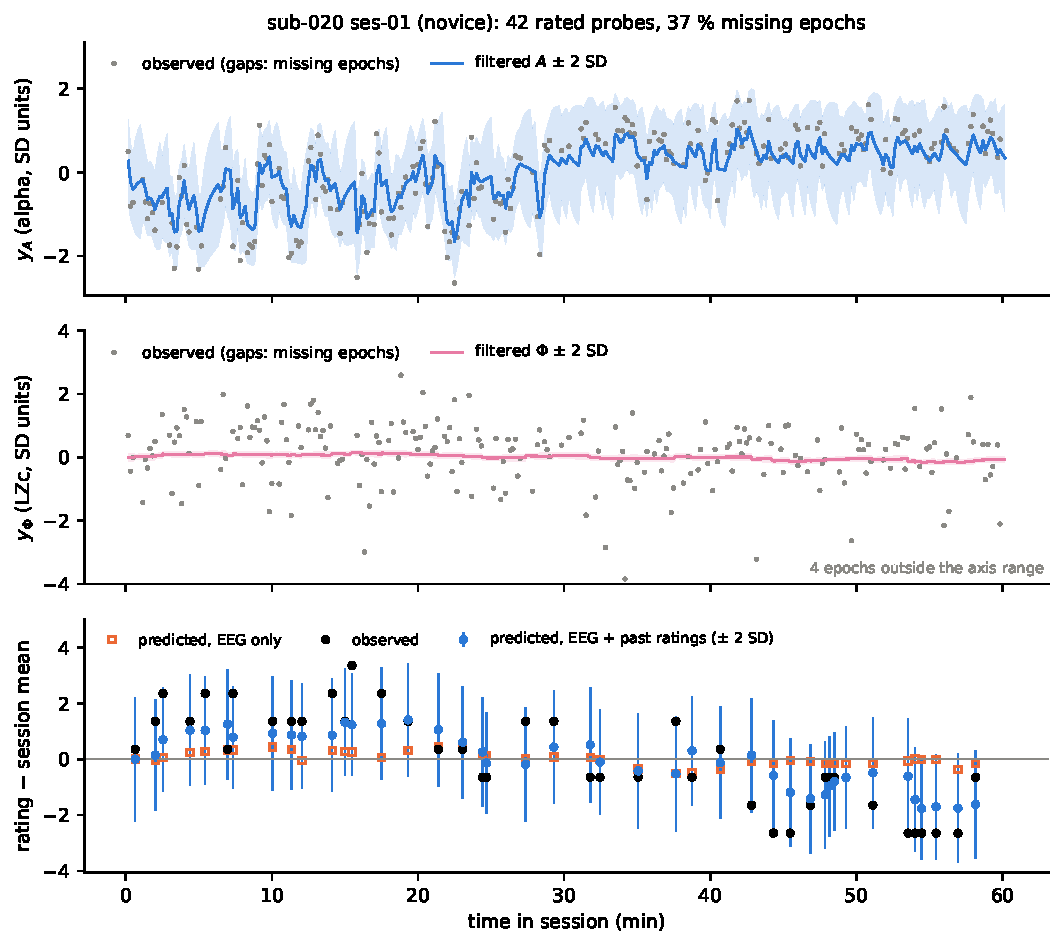
\includegraphics[width=0.49\textwidth]{fig9_realdata_session.pdf}\hfill
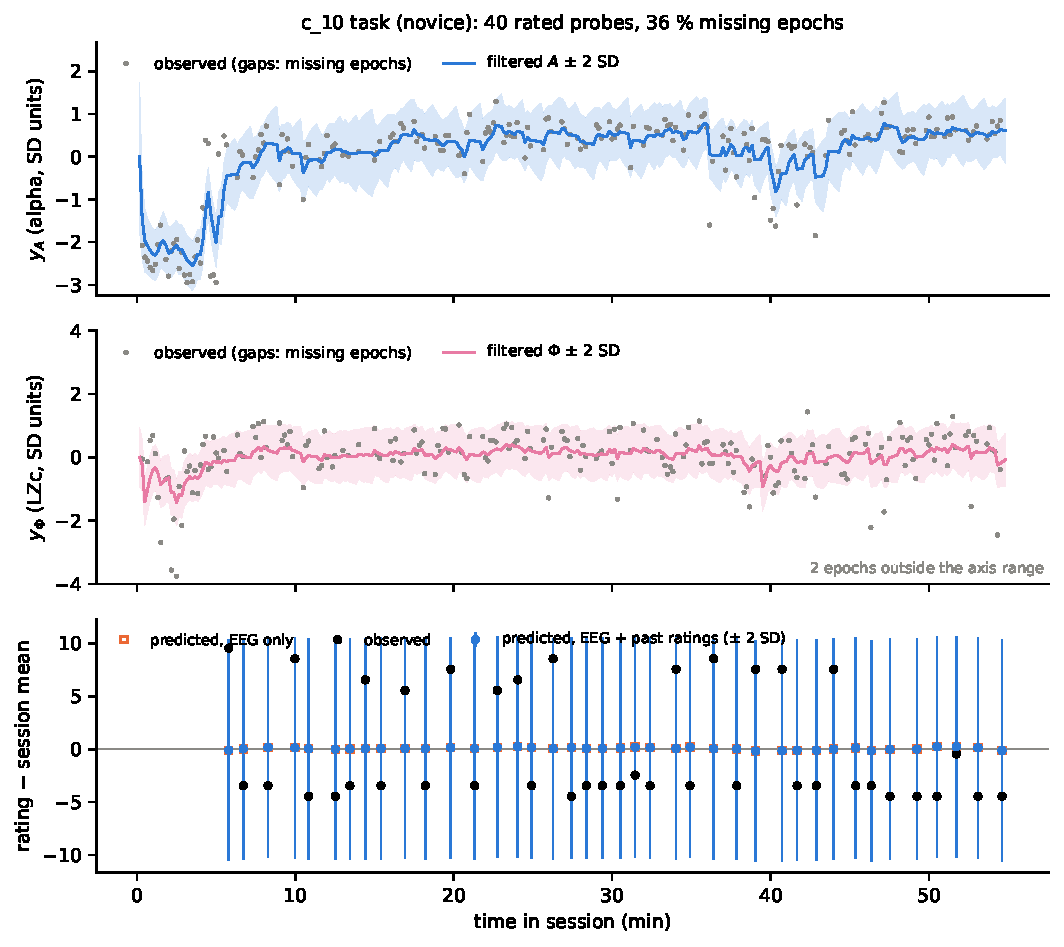
\includegraphics[width=0.49\textwidth]{fig11_osf_session.pdf}
\caption{\textbf{One retained session of each dataset filtered with M1 at the pooled estimate (in sample).} Left: ds001787, sub-020 ses-01 (novice); right: OSF 3uszv, c\_10 (novice); in each case the retained session with the most rated probes. Top: DMN proxy $y_A$ and the filtered $A\pm2$ SD. Middle: integration proxy $y_\Phi$ and the filtered $\Phi\pm2$ SD; on ds001787 the filtered $\Phi$ hardly moves because $y_\Phi$ is almost pure noise, on OSF 3uszv it fluctuates on a scale of tens of seconds; a few outlying epochs lie outside the axis. Bottom: ratings centred within session, with one-step-ahead predictions from EEG and past ratings ($\pm2$ SD) and from EEG alone. Gaps are missing epochs. On OSF 3uszv the alpha proxy drifts over minutes, with level shifts near 5 and 40~min, and the ratings alternate between about $+7$ and $-5$ without serial dependence, so that every prediction stays at the session mean.}
\label{fig:sessions}
\end{figure*}

\subsection{Predicted and Achieved Errors (RQ1)}
Fig.~\ref{fig:errors} is the main result. For the seven scale-free parameters of M1 it shows, on each dataset, the CRB computed before the lock, the Fisher standard error at the estimate, the bootstrap RMSE and the observed-information standard error. Table~\ref{tab:errors} gives the numbers for the two rate constants. On ds001787 the bound for $\kinh$ computed before any EEG was seen (9.1\,\%) and the bound recomputed on the retained sessions at the measured signal-to-noise ratio (13.3\,\%) bracket the 9.9\,\% achieved, and the bootstrap reproduces the Fisher value (ratio 0.98). On OSF 3uszv the denser probing and longer sessions give a smaller bound, 6.7\,\%, and the achieved Fisher error is 8.5\,\% with a bootstrap ratio of 1.03; the bootstrap-to-Fisher ratios are 0.98--1.69 on ds001787 and 1.00--1.08 on OSF 3uszv over all ten parameters, so gates E2 and F2 pass. Hypothesis H1 is supported under its preregistered Fisher criterion on both datasets. In Fisher terms the design analysis was accurate on ds001787 and somewhat optimistic on OSF 3uszv, where the achieved error exceeds the bound recomputed on the retained sessions by 15\,\%; both are well inside the factor of two with which the bound was validated in simulation.

\begin{figure*}[t]
\centering
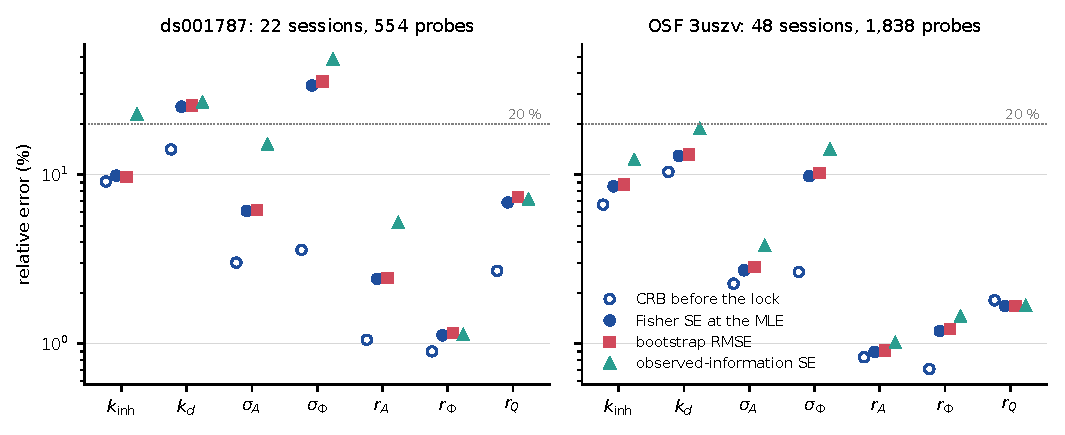
\includegraphics[width=0.95\textwidth]{fig1_pred_vs_achieved.pdf}
\caption{\textbf{Predicted and achieved relative errors of the scale-free parameters of M1 on the two datasets.} Open circles: Cram\'er--Rao bound from the exact Fisher information at the nominal parameters on the real probe schedules, computed before each lock. Filled circles: Fisher standard error at the maximum-likelihood estimate. Squares: root-mean-square error of 200 parametric-bootstrap refits. Triangles: standard error from the observed information (numerical Hessian). The dotted line is the 20\,\% criterion of hypothesis H1. For $\kinh$ the first three numbers agree on both datasets (largest over smallest 1.08 and 1.32); for $\kd$ the Fisher error exceeds the bound computed before the lock by a factor of 1.8 on ds001787 and 1.2 on OSF 3uszv; the observed-information error of the alpha-power channel ($\kinh$, $\sA$, $\rA$) exceeds the Fisher error by a factor of 2.1--2.5 on ds001787 and 1.1--1.4 on OSF 3uszv.}
\label{fig:errors}
\end{figure*}

\begin{table}[t]
\caption{\textbf{Three error numbers for the two rate constants (per minute), as relative errors in percent.} CRB: before the lock on all real designs, on the retained designs, and on these with $\rA$ at the measured signal-to-noise ratio. SE at the MLE: expected Fisher information, observed information, and profile likelihood. RMSE: 200 bootstrap refits; ratio: RMSE over Fisher SE (gate E2/F2).}
\label{tab:errors}
\centering\scriptsize
\setlength{\tabcolsep}{2.2pt}
\begin{tabular}{llrrrrrrrrr}
\toprule
 & & & \multicolumn{3}{c}{CRB} & \multicolumn{3}{c}{SE at the MLE} & & \\
\cmidrule(lr){4-6}\cmidrule(lr){7-9}
Dataset & Par. & Est. & lock & kept & SNR & Fisher & obs. & prof. & RMSE & ratio \\
\midrule
ds001787  & $\kinh$ & 1.32  & 9.1  & 12.3 & 13.3 & 9.9  & 22.8 & 21.9 & 9.7  & 0.98 \\
          & $\kd$   & 0.200 & 14.1 & 19.0 & 19.1 & 25.3 & 26.7 & 26.6 & 25.7 & 1.01 \\
OSF 3uszv & $\kinh$ & 0.140 & 6.7  & 7.4  & 7.4  & 8.5  & 12.2 & 11.8 & 8.8  & 1.03 \\
          & $\kd$   & 1.58  & 10.4 & 11.5 & 11.5 & 12.9 & 18.7 & 18.3 & 13.2 & 1.02 \\
\bottomrule
\end{tabular}
\end{table}

\subsection{The Misspecification Signature (RQ1)}
The observed information tells a different story for the DMN channel. On ds001787 the numerical Hessian gives 22.8\,\% for $\kinh$ and the profile likelihood 21.9\,\%, more than twice the Fisher value; the same factor, 2.1--2.5, appears for $\sA$ and $\rA$, whereas for $\kd$, $\rPhi$ and $\rQ$ observed and expected information agree within 6\,\%. On a dataset simulated from $\hat\thetav$ on the same 22 designs the factor for $\kinh$, $\sA$ and $\rA$ is 1.05--1.07. A gap confined to one channel and absent under the fitted model is the signature of misspecification of that channel: posterior alpha power is not fully described by one Ornstein--Uhlenbeck process plus white noise. On OSF 3uszv the signature is present but weaker, 1.43 for $\kinh$, 1.39 for $\sA$ and 1.13 for $\rA$ against 0.93--0.99 on simulated data, and it is no longer confined to the alpha channel (1.45 for $\kd$, 1.44 for $\sPhi$); the replication check R2, which required the factor to exceed 1.5, is not met. Fig.~\ref{fig:profiles} shows the profiles: on ds001787 the profile of $\kinh$ is about twice as wide as the Fisher quadratic while that of $\kd$ follows it; on OSF 3uszv the profiles of $\kinh$ and $\kd$ are 1.4 times wider than the quadratic, and the profile of $\kappa$ is asymmetric. Under the likelihood-based criterion H1 is therefore not supported on ds001787 (21.9\,\%, just above 20\,\%) and supported on OSF 3uszv (11.8\,\%). We report the profile interval as the uncertainty of $\kinh$ throughout.

\begin{figure*}[t]
\centering
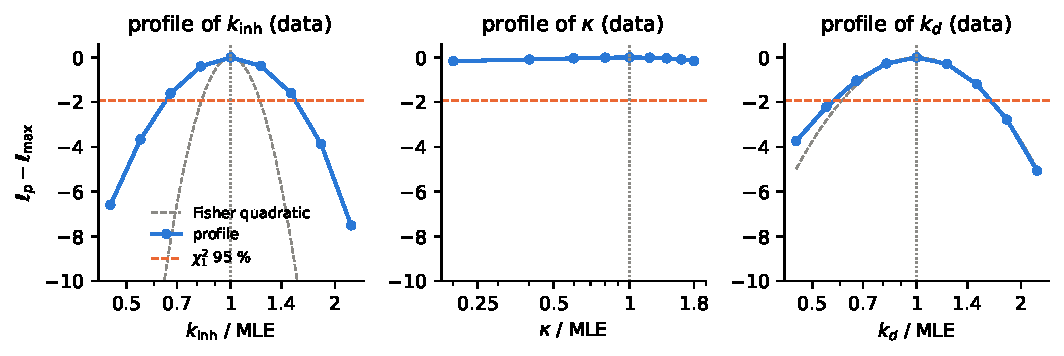
\includegraphics[width=0.82\textwidth]{fig10_realdata_profiles.pdf}\\[3pt]
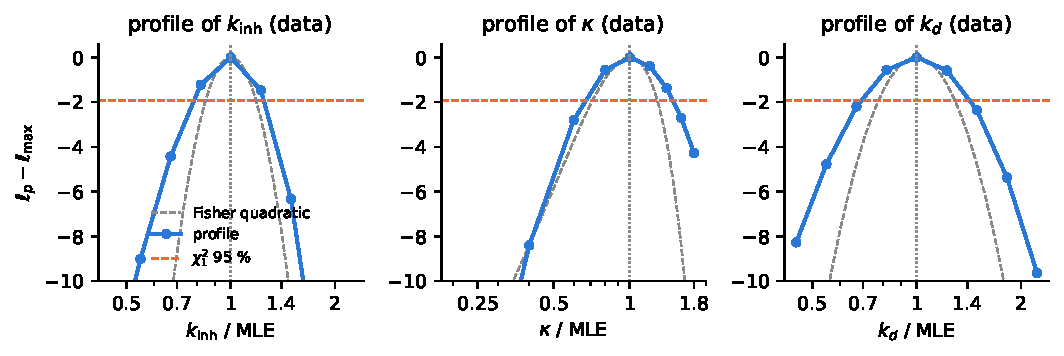
\includegraphics[width=0.82\textwidth]{fig12_osf_profiles.pdf}
\caption{\textbf{Profile log-likelihoods of the three rate constants, all other parameters re-optimised at each point.} Top: ds001787; bottom: OSF 3uszv. Grey dashed: quadratic approximation implied by the expected Fisher information at the maximum-likelihood estimate; orange: $\chi^2_1$ 95\,\% threshold. On ds001787 the profile of $\kinh$ is about twice as wide as the quadratic (95\,\% interval 0.86--2.02~min$^{-1}$), that of $\kd$ follows it, and that of $\kappa$ is flat because $\hat\kappa\approx0$. On OSF 3uszv the profile of $\kinh$ is 1.38 times wider than the quadratic (0.110--0.175~min$^{-1}$), that of $\kd$ 1.4 times, and the profile of $\kappa$, which is negative, is asymmetric ($-0.50$ to $-0.23$).}
\label{fig:profiles}
\end{figure*}

\subsection{Estimates}
Table~\ref{tab:compare} places the two fits side by side. On ds001787 the DMN proxy relaxes fast, $1/\hat k_{\mathrm{inh}}=0.76$~min (profile interval 0.49--1.17~min), against the nominal 5~min of the design analysis, and the latent integration variable slowly, $1/\hat k_d=5.0$~min (3.1--8.7~min); the coupling $\kappa$ is not distinguishable from zero. On OSF 3uszv the DMN proxy is slow, $1/\hat k_{\mathrm{inh}}=7.1$~min (5.7--9.1~min), nine times the ds001787 value, and the integration variable is fast, $1/\hat k_d=0.63$~min (0.45--0.91~min), eight times faster than before: the two time constants have exchanged places, and R1 fails by a factor of nine. The coupling is now determined and negative, $\hat\kappa=-0.33$ ($-0.50$ to $-0.23$). The proxies differ in quality between the datasets. On ds001787 the DMN channel has a signal-to-noise ratio of 1.11 against a nominal 1.58 and the integration channel 0.06 against a nominal 2.4: the spectrum-controlled complexity measure carries almost no slow signal. On OSF 3uszv the DMN channel has the nominal ratio (1.57) and the integration channel 0.54, eight times its ds001787 value.

\begin{table*}[t]
\caption{\textbf{The two preregistered fits side by side.} Time constants in minutes with 95\,\% profile intervals; gains with Fisher 95\,\% intervals and per unit of the within-session SD of the ratings (1.11 and 5.22). SE of $\kinh$: CRB before the lock, Fisher, observed information, profile likelihood. Obs/exp: observed over expected SE on the data (in parentheses: on data simulated from the fit). \mbox{\mathversion{normal}$\Delta$}LPD: out-of-sample log predictive density of M1 minus N2 (EEG only) and minus N1 (EEG and past ratings). Group difference: $\log\kinh$, experienced minus novice fit, Wald 95\,\% interval. Meta-analysis: random-effects $1/\kinh$ over the subjects with a finite SE and the between-subject SD $\tau$ of $\log\kinh$. Sensitivity: locked variants that keep the sign of $\alpha$, the sign of $\beta$ and the profile interval of $1/\kinh$.}
\label{tab:compare}
\centering\footnotesize
\setlength{\tabcolsep}{4pt}
\begin{tabular}{lll}
\toprule
 & ds001787 & OSF 3uszv \\
\midrule
Sessions retained / recorded; subjects   & 22 / 40; 16 & 48 / 58; 48 \\
Rated probes; probe interval; session    & 554; 1.6 min; 45 min & 1,838; 77 s; 57 min \\
Rating scale; within-session SD          & $-3$ to $3$; 1.11 & $-7$ to $7$; 5.22 \\
$1/\kinh$ (min)                          & 0.76 [0.49, 1.17] & 7.1 [5.7, 9.1] \\
$1/\kd$ (min)                            & 5.0 [3.1, 8.7] & 0.63 [0.45, 0.91] \\
$\kappa$                                 & $\approx0$, flat profile & $-0.33$ [$-0.50$, $-0.23$] \\
SNR of $y_A$; of $y_\Phi$                & 1.11; 0.06 & 1.57; 0.54 \\
SE of $\kinh$: CRB / Fisher / obs. / profile & 9.1 / 9.9 / 22.8 / 21.9\,\% & 6.7 / 8.5 / 12.2 / 11.8\,\% \\
Bootstrap RMSE / Fisher SE of $\kinh$    & 0.98 & 1.03 \\
Obs/exp SE: $\kinh$, $\sA$, $\rA$        & 2.30, 2.48, 2.14 (1.05--1.07) & 1.43, 1.39, 1.13 (0.93--0.99) \\
$\alpha$ [95\,\%]; per rating SD         & 13.1 [4.9, 21.3]; 11.8 & 0.79 [$-0.24$, 1.82]; 0.15 \\
$\beta$ [95\,\%]; per rating SD          & $-0.03$ [$-0.19$, 0.13]; $-0.02$ & 0.02 [$-0.34$, 0.38]; 0.00 \\
$\Delta$LPD vs N2; vs N1                 & $-0.010$; $-0.031$ & $+0.000$; $-0.001$ \\
Lag-1 autocorrelation of the ratings     & 0.22 & $-0.01$ \\
Group difference in $\log\kinh$          & $-1.19$ [$-1.56$, $-0.81$] & $+0.14$ [$-0.20$, 0.47] \\
Meta-analysis: $1/\kinh$; $\tau$; subjects & 0.95 [0.40, 2.26]; 1.19; 9 & 3.3 [2.0, 5.7]; 1.49; 35 \\
Ljung--Box median $p$: $y_A$, $y_\Phi$   & 0.27, 0.40 & 0.06, 0.42 \\
Sensitivity: $\alpha$, $\beta$, $1/\kinh$ kept & 6/6, 4/6, 4/6 & 5/6, 1/6, 4/6 \\
Gates                                    & E0--E3 passed & F0--F3 passed \\
\bottomrule
\end{tabular}
\end{table*}

\subsection{Gains and Out-of-Sample Prediction (RQ2)}
On ds001787 the gain from the integration variable to the rating is positive, $\hat\alpha=13.1$ (Fisher 95\,\% interval 4.9--21.3; no bootstrap replicate at or below zero), as hypothesis H3 predicted. Its meaning is limited: since $y_\Phi$ is essentially noise, the latent $\Phi$ is identified almost entirely by the ratings themselves, $\alpha$ and $\sPhi$ trade off (bootstrap correlation of $\log\sPhi$ and $\alpha$: $-0.83$), and only the contribution of $\Phi$ to the rating variance is well determined. On OSF 3uszv, where $\Phi$ is pinned by the complexity channel, $\hat\alpha=0.79$ with an interval that contains zero ($-0.24$ to $1.82$; 11 of 200 bootstrap replicates at or below zero): H3 is not supported. In units of the within-session rating SD the gain is 11.8 on ds001787 and 0.15 on OSF 3uszv. The DMN gain is $\hat\beta=-0.03$ ($-0.19$ to $0.13$) and $0.02$ ($-0.34$ to $0.38$): the sign asked for by H4 is not determined on either dataset, and posterior alpha power makes no detectable contribution to the ratings.

Table~\ref{tab:loso} gives the leave-one-session-out comparison of hypothesis H2. On ds001787, with EEG only, M1 predicts the ratings no better than the instantaneous regression N2; with EEG and past ratings it beats the running mean N3 but not the rating-only model N1, which has the best log predictive density and the smallest error of all models. The advantage over N3 therefore comes from the serial dependence of the reports (lag-1 autocorrelation 0.22), not from the EEG. On OSF 3uszv M1 is indistinguishable from N2 and N1 ($\Delta\mathrm{LPD}$ of $+0.0004$ and $-0.0006$), with a mean absolute error of 4.5--4.6 on a 14-point scale for every model but the running mean (4.7), and for a more basic reason: the ratings of this dataset have no serial dependence to predict (lag-1 autocorrelation $-0.01$), so past ratings do not help either, and their bimodal distribution is out of reach of a Gaussian read-out (Appendix~\ref{app:ppc}). H2 is not supported on either dataset.

\begin{table*}[t]
\caption{\textbf{Leave-one-session-out prediction of the ratings (hypothesis H2), (a) from EEG only and (b) from EEG and past ratings.} LPD: mean Gaussian log predictive density per probe; MAE: mean absolute error. \mbox{\mathversion{normal}$\Delta$}LPD: M1 minus null model with a session-level bootstrap 95\,\% interval. N2: instantaneous regression on $(y_A,y_\Phi)$; N1: M1 with the rating channel only; N3: running mean of past ratings.}
\label{tab:loso}
\centering\footnotesize
\setlength{\tabcolsep}{5pt}
\begin{tabular}{llrrrrr}
\toprule
 & Comparison & LPD M1 & LPD null & $\Delta$LPD [95\,\%] & MAE M1 & MAE null \\
\midrule
ds001787 & (a) vs N2 & $-1.546$ & $-1.541$ & $-0.010$ [$-0.039$, $0.017$] & 0.93 & 0.92 \\
(554 probes) & (b) vs N1 & $-1.472$ & $-1.421$ & $-0.031$ [$-0.103$, $0.009$] & 0.88 & 0.84 \\
 & (b) vs N3 & $-1.472$ & $-1.626$ & $+0.154$ [$0.083$, $0.233$] & 0.88 & 1.00 \\
\midrule
OSF 3uszv & (a) vs N2 & $-3.0746$ & $-3.0749$ & $+0.0004$ [$-0.0006$, $0.0014$] & 4.54 & 4.56 \\
(1,838 probes) & (b) vs N1 & $-3.0746$ & $-3.0740$ & $-0.0006$ [$-0.0018$, $0.0006$] & 4.54 & 4.55 \\
 & (b) vs N3 & $-3.0746$ & $-3.1445$ & $+0.0712$ [$0.0609$, $0.0815$] & 4.54 & 4.66 \\
\bottomrule
\end{tabular}
\end{table*}

\subsection{Groups and Subjects}
On ds001787, fitted separately, the experienced group has a smaller $\kinh$ than the novices (log difference $-1.19$, Wald 95\,\% interval $-1.56$ to $-0.81$), opposite to hypothesis H5. The two separate fits differ mainly in how the alpha-power variance is split between state and observation noise (signal-to-noise ratio 1.05 against 2.23), and $\kinh$ trades off against that split: when all other parameters are shared the log difference shrinks to $-0.18$ and the preregistered one-degree-of-freedom test is not significant ($\chi^2_1=3.3$, $p=0.068$), although the groups differ in some parameter ($\chi^2_{10}=41$). The groups also differ in sex and age (10 of 12 against 2 of 12 men, mean age 39 against 48 years). On OSF 3uszv, with 25 and 23 sessions, the group fits give $\hat k_{\mathrm{inh}}=0.154$ and $0.134~\mathrm{min^{-1}}$, a log difference of $+0.14$ ($-0.20$ to $0.47$; $\chi^2_1=2.67$, $p=0.10$), below the minimal detectable difference of 0.37: neither F-H5a nor F-H5b is supported, and the difference found on ds001787 does not recur. The groups differ in other parameters ($\chi^2_{10}=256$): in the novices the integration variable is fast and noisy ($1/\kd=0.33$~min, $\sPhi=1.1$) and loads positively on the reports ($\alpha=2.0$, $\beta=+0.75$); in the experienced practitioners it is slower ($1/\kd=0.89$~min, $\sPhi=0.68$) and both gains are near zero or negative ($\alpha=-0.15$, $\beta=-0.66$). Per-subject fits gave finite standard errors for 9 of 16 subjects on ds001787 and 35 of 48 on OSF 3uszv (for most of the others $\sPhi$ was estimated at zero). Their meta-analyses give DMN time constants of 0.95~min (0.40--2.26) and 3.3~min (2.0--5.7) with between-subject standard deviations of $\log\kinh$ of 1.19 and 1.49 log units ($I^2=0.92$ on both): the pooled fits describe an average practitioner at best.

\subsection{Model Checks and Sensitivity}
The innovations are close to white on ds001787 (median Ljung--Box $p=0.27$ for $y_A$ and $0.40$ for $y_\Phi$; four of 22 sessions below 0.01 for $y_A$) and less so on OSF 3uszv ($p=0.058$ for $y_A$, with 17 of 48 sessions below 0.01; $0.42$ for $y_\Phi$); the innovations of the two channels are uncorrelated on both (median 0.05), so the diagonal observation noise was kept. The posterior predictive check (Appendix~\ref{app:ppc}) reproduces the serial dependence of the ds001787 ratings (lag-1 autocorrelation 0.22, simulated 0.26, band 0.15--0.37) and the absence of serial dependence on OSF 3uszv ($-0.01$; simulated $-0.03$, band $-0.08$ to $0.02$), but not the skewed centre of the ds001787 distribution nor the bimodal OSF distribution, and on both datasets the experienced practitioners rate with a smaller spread than the pooled model implies (OSF: observed difference in within-session SD $-1.01$, simulated $-0.31$, band $-0.55$ to $-0.05$).

Table~\ref{tab:sens} lists the sensitivity analyses. On ds001787 $\alpha$ stays positive in all six locked variants, the sign of $\beta$ is kept in four, and $1/\kinh$ stays inside the profile interval in four: the frontal-theta proxy gives 4.0~min, and the variant with at most 20\,\% missing epochs keeps two sessions and is degenerate. On OSF 3uszv that variant retains no session, because the probe windows alone exceed 20\,\% in every session, an oversight of the preregistration, so six variants run; the sign of $\alpha$ is kept in five (it is negative with the aperiodic-exponent proxy), the sign of $\beta$ in one, and $1/\kinh$ stays inside the interval in four (frontal theta gives 17~min and per-session z-scoring 4.8~min). The 80\,\% rule is therefore met for the sign of $\alpha$ on both datasets and for nothing else, and the estimates are reported descriptively. One post-registration variant on OSF 3uszv, added after Fig.~\ref{fig:sessions} had been examined, masks the EEG before the first probe (the sessions begin with instructions and a practice probe, and the first bell comes after 6.8~min on average): the DMN time constant rises from 7.1 to 16~min, so the level shift of alpha at the start of the session is the fastest part of this proxy.

\begin{table*}[t]
\caption{\textbf{Sensitivity analyses: pooled estimates with time constants in minutes.} The fixed 150~$\mu$V rule is the locked primary rule of ds001787 and a locked variant of OSF 3uszv; the adaptive rule is a post-registration variant of ds001787 and the locked primary rule of OSF 3uszv. The last row is a post-registration variant and does not count in the robustness rule. On ds001787 the variant with at most 20\,\% missing epochs retains two sessions and is degenerate; on OSF 3uszv it retains none.}
\label{tab:sens}
\centering\footnotesize
\setlength{\tabcolsep}{5pt}
\begin{tabular}{lrrrrrrrr}
\toprule
 & \multicolumn{4}{c}{ds001787} & \multicolumn{4}{c}{OSF 3uszv} \\
\cmidrule(lr){2-5}\cmidrule(lr){6-9}
Variant & $n$ & $\alpha$ & $\beta$ & $1/\kinh$ & $n$ & $\alpha$ & $\beta$ & $1/\kinh$ \\
\midrule
Primary analysis                     & 22 & 13.10 & $-0.026$ & 0.76 & 48 & 0.79 & $+0.018$ & 7.12 \\
$y_A$: periodic alpha                & 22 & 13.10 & $-0.069$ & 0.52 & 48 & 0.79 & $+0.069$ & 7.74 \\
$y_A$: frontal theta                 & 22 & 13.08 & $-0.389$ & 3.98 & 48 & 0.76 & $-0.293$ & 16.76 \\
$y_\Phi$: negative aperiodic exponent & 22 & 13.08 & $+0.045$ & 0.76 & 48 & $-0.10$ & $-0.127$ & 7.91 \\
Per-session z-score                  & 22 & 13.10 & $-0.051$ & 0.90 & 48 & 0.82 & $-0.108$ & 4.81 \\
At most 20\,\% missing epochs        &  2 & 399.6 & $-0.239$ & 0.23 &  0 & -- & -- & -- \\
First 20 probes                      & 22 & 13.09 & $+0.096$ & 0.76 & 48 & 1.43 & $-0.096$ & 7.10 \\
Fixed 150~$\mu$V rule                & \multicolumn{4}{c}{(primary)} & 24 & 0.36 & $-0.470$ & 5.74 \\
Adaptive rule                        & 39 & 0.97 & $+0.215$ & 0.48 & \multicolumn{4}{c}{(primary)} \\
EEG masked before the first probe    & -- & -- & -- & -- & 48 & 1.02 & $+0.285$ & 16.00 \\
\bottomrule
\end{tabular}
\end{table*}

\subsection{Comparison With the Parameters of BQI (RQ3)}
\label{sec:res-bqi}
Table~\ref{tab:bqi} sets the estimates beside the predictions T1--T5 of BQI (Section~\ref{sec:theory-pred}) and the values that BQI fitted to meta-analytic data \cite[Table~5]{BQI}. The time constants are scale-free and can be compared directly; the coupling and the gains depend on the units of the standardised proxies and of the rating scales, so only their signs can be compared. Neither dataset reproduces the BQI time constants: the DMN time constant is 0.76 and 7.1~min against 23~min, and the integration time constant 5.0 and 0.63~min against 29~min, with the BQI values outside all four profile intervals. The coupling, positive in \cite[eq.~(53)]{BQI}, is indistinguishable from zero on ds001787 and negative on OSF 3uszv. The gain $\alpha$ is positive on both datasets, as in BQI, but its interval excludes zero only on ds001787; the sign of $\beta$, positive in BQI, is undetermined on both; and the group difference that follows from \cite[eq.~(51) and Sec.~7.5]{BQI} is reversed on ds001787 and absent on OSF 3uszv. Of the five predictions, only T3 is reproduced in sign, and with a determined sign only on ds001787.

\begin{table*}[t]
\caption{\textbf{Parameter values of BQI and the estimates on the two datasets.} BQI: least-squares fit to meta-analytic data \cite[Table~5]{BQI}. Time constants in minutes with 95\,\% profile intervals; $\kappa$ with its profile interval; gains with Fisher 95\,\% intervals; group difference of $\log\kinh$ (experienced minus novice) with the Wald interval. The coupling and the gains are in the units of the standardised proxies and ratings, so only their signs are comparable with BQI.}
\label{tab:bqi}
\centering\footnotesize
\setlength{\tabcolsep}{5pt}
\begin{tabular}{llll}
\toprule
Quantity & BQI & ds001787 & OSF 3uszv \\
\midrule
$1/\kinh$ (min) & 23 & 0.76 [0.49, 1.17] & 7.1 [5.7, 9.1] \\
$1/\kd$ (min) & 29 & 5.0 [3.1, 8.7] & 0.63 [0.45, 0.91] \\
Sign of $\kappa$ & $+$ & $\approx0$, flat profile & $-$ ($-0.33$ [$-0.50$, $-0.23$]) \\
Sign of $\alpha$ & $+$ (2.34) & $+$ (13.1 [4.9, 21.3]) & $+$, undetermined (0.79 [$-0.24$, 1.82]) \\
Sign of $\beta$ & $+$ (1.87) & undetermined & undetermined \\
Experienced $-$ novice, $\log\kinh$ & $>0$ & $-1.19$ [$-1.56$, $-0.81$] & $+0.14$ [$-0.20$, 0.47] \\
\bottomrule
\end{tabular}
\end{table*}

\subsection{What Replicates (RQ4)}
Table~\ref{tab:tests} lists every preregistered hypothesis and check with its outcome. Three findings are common to the two datasets and two are not. (i) The Fisher-based error numbers were accurate on both: for $\kinh$ the bound computed before the lock, the Fisher SE at the estimate and the bootstrap RMSE differ by at most 8\,\% on ds001787 and 32\,\% on OSF 3uszv, and on both the likelihood-based SE of the alpha channel exceeds the Fisher SE. (ii) Neither EEG proxy improves the out-of-sample prediction of the reports on either dataset. (iii) The between-subject heterogeneity of $\log\kinh$ is large on both ($\tau$ of 1.2 and 1.5). (iv) $\alpha>0$ does not replicate: the estimate is positive on both, but the interval excludes zero only on ds001787, and on both its value per rating SD says little. (v) The rate constants themselves do not replicate: $1/\kinh$ is 0.76~min on ds001787 and 7.1~min on OSF 3uszv, $1/\kd$ is 5.0 against 0.63~min, and the direction of the group difference differs.

\begin{table*}[t]
\caption{\textbf{Preregistered hypotheses and replication checks with their outcomes on the two datasets (intervals are 95\,\%).}}
\label{tab:tests}
\centering\footnotesize
\setlength{\tabcolsep}{3pt}
\begin{tabular}{lll}
\toprule
Hypothesis & ds001787 & OSF 3uszv \\
\midrule
H1: SE of $\kinh$ at most 20\,\% & Fisher 9.9\,\% (profile 21.9\,\%): supported (Fisher) & Fisher 8.5\,\% (profile 11.8\,\%): supported \\
H2: M1 beats null models & $\Delta$LPD $-0.010$ (N2), $-0.031$ (N1): not supported & $+0.0004$ (N2), $-0.0006$ (N1): not supported \\
H3: $\alpha>0$ & 13.1 [4.9, 21.3]: supported & 0.79 [$-0.24$, 1.82]: not supported \\
H4: sign of $\beta$ & $-0.03$ [$-0.19$, 0.13]: undetermined & 0.02 [$-0.34$, 0.38]: undetermined \\
H5: $\kinh$ higher in experts & $-1.19$ [$-1.56$, $-0.81$]; LR $p=0.068$: not supported & $+0.14$ [$-0.20$, 0.47]; LR $p=0.10$: not supported (a, b) \\
R1: $1/\kinh$ in 0.49--1.17 min & -- & 7.1 min [5.7, 9.1]: not replicated \\
R2: obs/exp SE $>1.5$, $\approx1$ simulated & 2.30; 1.05 & 1.43; 0.93: not replicated \\
R3: $1/\kd$ & 5.0 min [3.1, 8.7] & 0.63 min [0.45, 0.91] \\
\bottomrule
\end{tabular}
\end{table*}

\subsection{Why the Time Constants Differ: A Simulation}
The exchange of the two time constants has a simple reading. On ds001787 the complexity proxy was noise, so $\Phi$ and $\kd$ were identified by the ratings and $1/\kd$ measured the slow drift of the reports; on OSF 3uszv the complexity proxy carries a 40-s signal that fixes $\Phi$, the reports have no drift, and the alpha proxy drifts over minutes within hour-long sessions (Fig.~\ref{fig:sessions}). Fig.~\ref{fig:sim} shows what an Ornstein--Uhlenbeck fit does with such a feature. When the feature is the sum of a fast component (0.5~min) and a slow one (3, 7 or 15~min), the fitted time constant moves monotonically from the fast to the slow value as the slow component's share of the variance grows: with equal shares the fit returns 1.2, 1.7 and 1.9~min, and the slow value is reached only when the slow component carries nearly all of the variance (at a share of 0.8, a 7-min component gives 3.6~min and a 15-min component 7.5~min). A single rate constant estimated from an uncalibrated feature is therefore a variance-weighted summary of whatever time scales that feature contains in that recording, which depends on the montage, the session length and the practice; the frontal-theta alternative gives 4~min on one dataset and 17~min on the other for the same reason. The DMN time constant of M1 is a property of the feature, not yet of a DMN process.

\begin{figure}[t]
\centering
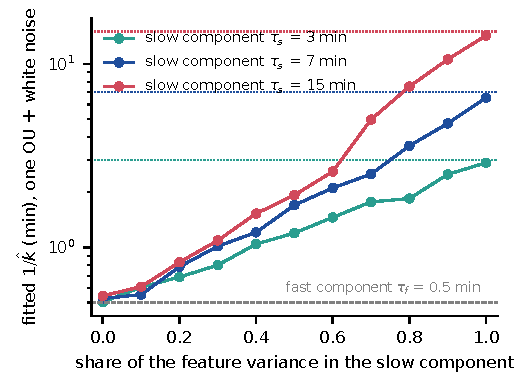
\includegraphics[width=\columnwidth]{fig2_ou_timescale.pdf}
\caption{\textbf{An Ornstein--Uhlenbeck fit returns the dominant time scale of the feature it is given.} A simulated feature is the sum of a fast component ($\tau_f=0.5$~min), a slow component ($\tau_s$ of 3, 7 or 15~min, dotted lines) and white noise, on the OSF 3uszv design (48 sessions of 57~min with probe windows and 10\,\% further epochs missing). It is fitted with one Ornstein--Uhlenbeck process plus white noise, the DMN channel of M1. The fitted time constant moves from $\tau_f$ to $\tau_s$ as the slow component's share of the feature variance grows.}
\label{fig:sim}
\end{figure}

%% VI. Discussion: interpretation by research question, implications, limitations. Input by access.tex.
\section{Discussion}
\label{sec:discussion}

\subsection{What the Design Analysis Got Right (RQ1)}
The companion paper promised that the exact Fisher information of M1 could be used to plan an experience-sampling study. On two real designs, with irregular probes, a third of the epochs missing and sessions excluded by an artefact rule, the bound computed before the lock, the Fisher standard error at the estimate and the bootstrap error of $\kinh$ differed by at most 8\,\% on ds001787 and 32\,\% on OSF 3uszv. On ds001787 the achieved 9.9\,\% lay between the bound computed before the lock and the bound recomputed at the measured signal-to-noise ratio (9.1--13.3\,\%); on OSF 3uszv the achieved 8.5\,\% exceeded the recomputed bound (7.4\,\%) by 15\,\%. For $\kd$ the bound computed before the lock was optimistic by a factor of 1.8 and 1.2. The ordering between the datasets was also predicted: the denser probing and longer sessions of OSF 3uszv give a smaller bound and a smaller achieved error. A design analysis of this kind can therefore be used for its intended purpose, deciding how many subjects, how long a session and how many probes are needed, provided the error it quotes is understood as a Fisher error of a model assumed to be right.

\subsection{What It Cannot Anticipate (RQ1)}
A bound cannot anticipate misspecification, and the alpha-power channel is misspecified on both datasets: the observed-information and profile errors of $\kinh$, $\sA$ and $\rA$ exceed the Fisher error by a factor of 2.1--2.5 on ds001787 and 1.1--1.4 on OSF 3uszv, and the excess disappears on data simulated from the fit. The diagnostic is cheap, since it needs one Hessian and one simulated dataset, and we recommend it alongside the bootstrap, which cannot see misspecification because it simulates from the model. In practice, design-map numbers should be read as lower bounds whenever a proxy is not known to follow the model, and likelihood-based intervals should be reported beside Fisher-based ones; on ds001787 the two criteria for H1 disagree.

\subsection{The Observation Model Is the Bottleneck (RQ2)}
The two proxies we preregistered carried no detectable information about the reports beyond the reports' own serial dependence, on either dataset. The complexity channel was noise on ds001787 and, on OSF 3uszv, a 40-s signal unrelated to the reports; posterior alpha did not load on the ratings on either. The dynamics of M1 are identifiable and were estimated with the predicted precision, but the read-out from EEG features to the reported state is where the information is missing. This is consistent with the indirect relation between posterior alpha and the DMN found in simultaneous EEG--fMRI \cite{Laufs2003,Mantini2007}. Finding an EEG feature that tracks the reported state, with a signal-to-noise ratio in the range that the design analysis shows to be necessary, is the open problem that this class of models leaves to experimenters, and the experience-sampling datasets now available \cite{Weinstein2018,Brandmeyer2018,RodriguezLarios2021} are the place to look for it.

\subsection{Implications for the BQI Framework (RQ3)}
Neither dataset supports the predictions T1, T2, T4 and T5 of BQI, and T3 holds in sign only (Section~\ref{sec:res-bqi}), but the comparison is not like for like. The BQI values were fitted to meta-analytic summaries of fMRI contrasts and cross-sectional correlations \cite[Sec.~7.2--7.5]{BQI}, a limitation that BQI itself states \cite[Sec.~11.3]{BQI}, whereas the present estimates come from EEG proxies observed over minutes within single sessions. A time constant fitted to meta-analytic group summaries describes at most how group-level DMN contrasts evolve over a practice; the 0.76 and 7.1~min estimated here describe how posterior alpha power fluctuates around its session mean. Because the Ornstein--Uhlenbeck DMN of M1 is the quadratic-potential case of the BQI Langevin dynamics \cite[eqs.~(83)--(87)]{BQI}, the estimated $\kinh$ is the curvature of that potential for the EEG proxy, not for the DMN itself. The negative coupling on OSF 3uszv says that, with posterior alpha standing in for the DMN, alpha and complexity rise together, the opposite of the coupling in \cite[eq.~(53)]{BQI}; it does not refute that eq.~(53) holds for the DMN itself. What the comparison shows is the step that BQI leaves open: before its parameters can be estimated from EEG, the EEG features must be calibrated against the state variables, for instance with the simultaneous EEG, fMRI and complexity recordings that BQI itself proposes \cite[Sec.~14]{BQI}, and the QoC must be operationalised with a validated instrument. The structural parts of BQI that M1 keeps, an Ornstein--Uhlenbeck DMN process feeding an integration variable and a linear read-out to the report, were estimable on both datasets with the precision the design analysis predicted.

\subsection{Rate Constants Are Properties of the Proxy (RQ4)}
The replication separates two kinds of result. The methodological ones held across laboratories: predicted and achieved errors of $\kinh$ agreed to within a third, the alpha channel showed the same signature, the EEG added nothing to prediction, and the heterogeneity between practitioners was large. The substantive ones did not: the DMN time constant moved from 0.8 to 7~min, the integration time constant from 5 to 0.6~min, and the group difference in $\kinh$ that ds001787 had shown disappeared. The simulation of Section~\ref{sec:simmethods} shows that this is expected rather than puzzling. An Ornstein--Uhlenbeck fit returns a variance-weighted compromise between the time scales present in the feature; posterior alpha power in a 45-min mantra session and in a 60-min breath-focus session, recorded with different montages, need not contain the same mixture. The lesson is not that one of the two estimates is wrong but that a rate constant estimated from an uncalibrated proxy is a property of the proxy in that recording. The parameters that a design analysis can promise to deliver are only as meaningful as the mapping from features to state variables, and that mapping must be established and shown to be stable across laboratories before a design map is used to plan a study or a closed-loop intervention \cite{Sitaram2017,Ros2020}: the control gains computed in the companion paper assume parameters that mean something.

\subsection{What the Preregistration Caught}
Two episodes illustrate the value of locks and gates. The locked artefact rule of ds001787 excluded 45\,\% of the sessions, which the stop criterion allowed; without the lock the natural reaction would have been to switch to the adaptive rule, which gives a different integration time constant and a positive $\beta$, and to report that. On OSF 3uszv a sensitivity variant copied from the first preregistration could not run, and 17 sessions were first preprocessed on a machine without the ICLabel package, which the preprocessing logs recorded; they were reprocessed before any fit was reported, and both facts are listed in Appendix~\ref{app:deviations}. Preregistration did not make the analysis simpler, but it made the list of what was decided after seeing the data short and explicit \cite{Nosek2018}.

\subsection{Limitations}
\label{sec:limitations}
The empirical tests are two datasets whose rate constants disagree by factors of eight and nine. On ds001787 the preregistered artefact rule excluded 18 of 40 sessions non-randomly, and the group comparison is confounded by sex and age; on OSF 3uszv the probe windows alone remove a third of the EEG, the ratings are bimodal and serially independent, and the sessions include an initial segment before the first probe whose masking doubles the DMN time constant. On both, the EEG features are proxies without a calibrated mapping to $A$ or $\Phi$ (posterior alpha is not a measure of DMN activity, Lempel--Ziv complexity is not a measure of $\Phi$), the levels $A_0$, $\Phi^*$ and $\gamma_0$ are not estimable after centring, and the alpha channel shows signs of misspecification. The two rating scales are operational stand-ins for the QoC of BQI rather than validated measures of it, and the complexity proxy, like the index of BQI, measures complexity rather than integration \cite[Sec.~11.3]{BQI}. M1 is linear with Gaussian noise and a linear read-out, whereas the ratings are ordinal and bounded, bimodal on one dataset, and meditation dynamics may involve discrete state switches \cite{Hasenkamp2012,Christoff2016}; non-linear extensions would require approximate filters. Subjects share one parameter vector in the pooled fits, although the between-subject standard deviation of $\log\kinh$ is 1.2--1.5 log units; a hierarchical model is the natural next step and would change the design map quantitatively. Finally, the analysis was planned, locked and run by a single author, and the preregistrations were not reviewed before the lock.

%% VII. Conclusion and future work. Input by access.tex.
\section{Conclusion}
\label{sec:conclusion}
Under two locked preregistrations and eight verification gates, a linear-Gaussian state-space model of meditation dynamics, derived from the BQI framework, was fitted to experience-sampling EEG from two laboratories. On the four research questions: (RQ1) the precision predicted by an exact Fisher-information design analysis before the EEG was seen was achieved on ds001787 and missed by 28\,\% on OSF 3uszv (8.5 against 6.7 percent for the DMN rate), well inside the factor of two with which the bound was validated in simulation, although the observed-information and profile errors expose a misspecified alpha-power channel; (RQ2) neither EEG proxy carries information about the reports beyond their own serial dependence; (RQ3) of the five predictions of BQI for the estimated quantities (Section~\ref{sec:theory-pred}), only the positive sign of $\alpha$ is reproduced, with a determined sign on ds001787 alone, while the time constants, the coupling, the sign of $\beta$ and the group difference are not; and (RQ4) the rate constants, estimated from uncalibrated proxies, are properties of the feature in the recording rather than of a brain process, so they do not transfer between laboratories. This is the first empirical support for using such a design analysis to plan experience-sampling studies, and a demonstration of what it cannot promise. Design analyses of dynamical models of mental states should therefore be read as statements about precision, be accompanied by observed-information and profile errors, and be preceded by a calibration of the features that is shown to hold across recordings.

Three lines of future work follow. First, a calibration study that records EEG together with fMRI and a complexity index, as BQI proposes \cite[Sec.~14]{BQI}, would establish which EEG feature, if any, tracks DMN activity and integration well enough for the design analysis to apply. Second, a hierarchical state-space model with subject-level rate constants would address the large between-subject heterogeneity and change the design map quantitatively. Third, a non-linear or ordinal read-out would match the bounded and, on one dataset, bimodal ratings, at the price of approximate filters and simulation-based Fisher information.

%% VIII. Appendices A (deviations), B (posterior predictive checks), C (reproduction). Input by access.tex.
\appendices

\section{Deviations From the Preregistrations}
\label{app:deviations}
\textit{ds001787.} (i) The amplitude survey and the post-registration adaptive artefact rule described in Section~\ref{sec:methods}. (ii) The locked text specifies ICLabel at 0.8; because ICLabel was trained on extended-infomax decompositions of 1--100~Hz data, the decomposition was computed on a 1--100~Hz copy of each cleaned recording, whose content ends at the 52~Hz anti-aliasing limit of the amplifier, and applied to the 1--40~Hz data. (iii) The code for the interval of the group difference and the one-degree-of-freedom test of E-H5 was completed after the pooled fit; both tests are those specified before the lock. (iv) Seven of 16 subjects were excluded from the meta-analysis by the non-finite-standard-error rule fixed in the code before fitting. (v) The standard error from the observed information, bootstrap percentile intervals, profile intervals and the CRB at the measured signal-to-noise ratio were added as descriptive quantities. (vi) The locked text announces five sensitivity analyses but lists six variants, so the robustness rule is applied as a fraction, 80\,\%; ``unchanged'' is taken to mean inside the 95\,\% profile interval of the primary analysis. (vii) The exploratory analyses listed in the preregistration (drowsiness as a covariate, within-session trends, between-session differences within subjects, an age- and sex-adjusted group comparison) are not reported.

\textit{OSF 3uszv.} (i) The variant restricted to sessions with at most 20\,\% missing epochs retains no session: with a probe every 77~s and a response of 17~s on average, the epochs that overlap a probe window make up 28--39\,\% of every session; the robustness rule is applied to the six variants that run. (ii) $\kappa$ is estimated negative, and the profile interval of a parameter with a free sign is taken on the linear grid rather than the log grid used for the rates. (iii) Seventeen of the 58 sessions (all novices) were first preprocessed on a machine on which ICLabel could not be imported, so that the documented fallback heuristic rejected a median of 6 components instead of 2; they were reprocessed with ICLabel before any fit, and every number reported here uses the reprocessed features. (iv) Thirteen of 48 subjects were excluded from the meta-analysis by the non-finite-standard-error rule (11 with $\sPhi$ at zero). (v) The post-registration variant that masks the EEG before the first probe was added after Fig.~\ref{fig:sessions} had been examined; it is reported separately. The exploratory analyses (sleepiness as a covariate, depth of focus in place of confidence, within-session trends) are not reported.

\section{Posterior Predictive Checks of the Ratings}
\label{app:ppc}
Tables~\ref{tab:ppc1} and \ref{tab:ppc2} compare the observed frequency of each rating level with ratings simulated from $\hat\thetav$ on the real designs (200 replicates, session means added back, rounded and clipped to the scale). On ds001787 the Gaussian read-out reproduces the extreme levels but places too much mass at 0 and too little at $+1$. On OSF 3uszv the data are bimodal and the Gaussian read-out is not.

\begin{table*}[t]
\caption{\textbf{Posterior predictive check on ds001787 (22 sessions): frequency of each rating level in percent.}}
\label{tab:ppc1}
\centering\footnotesize
\setlength{\tabcolsep}{6pt}
\begin{tabular}{lrrrrrrr}
\toprule
Level & $-3$ & $-2$ & $-1$ & $0$ & $+1$ & $+2$ & $+3$ \\
\midrule
Observed   & 3.4 & 7.8 & 15.9 & 18.6 & 29.2 & 18.4 & 6.7 \\
Simulated  & 2.0 & 7.6 & 17.8 & 24.7 & 23.5 & 15.7 & 8.7 \\
95\,\% band & 0.9--3.6 & 4.9--10.5 & 14.1--21.8 & 20.6--28.7 & 19.3--27.1 & 12.1--19.5 & 5.6--12.3 \\
\bottomrule
\end{tabular}
\end{table*}

\begin{table*}[t]
\caption{\textbf{Posterior predictive check on OSF 3uszv (48 sessions): frequency of each rating level in percent; the level 0 cannot occur in the data.}}
\label{tab:ppc2}
\centering\footnotesize
\setlength{\tabcolsep}{6pt}
\begin{tabular}{lrrrrrrrr}
\toprule
Level & $-7$ & $-6$ & $-5$ & $-4$ & $-3$ & $-2$ & $-1$ & $0$ \\
\midrule
Observed   & 12.6 & 11.3 & 5.4 & 2.0 & 1.5 & 0.5 & 1.0 & 0.0 \\
Simulated  & 7.0 & 2.7 & 3.4 & 4.1 & 4.9 & 5.6 & 6.1 & 6.7 \\
95\,\% band & 5.8--8.0 & 2.0--3.5 & 2.7--4.2 & 3.2--5.1 & 4.0--5.8 & 4.5--6.7 & 5.2--7.2 & 5.6--8.1 \\
\midrule
Level & $+1$ & $+2$ & $+3$ & $+4$ & $+5$ & $+6$ & $+7$ & \\
\midrule
Observed   & 1.3 & 0.9 & 1.7 & 4.5 & 11.8 & 19.8 & 25.8 & \\
Simulated  & 6.9 & 7.0 & 6.9 & 6.6 & 6.0 & 5.4 & 20.8 & \\
95\,\% band & 5.8--8.0 & 5.8--8.3 & 5.8--7.9 & 5.5--7.7 & 5.1--7.2 & 4.4--6.5 & 19.1--22.9 & \\
\bottomrule
\end{tabular}
\end{table*}

\section{Reproduction}
\label{app:repro}
Each dataset runs in gate order; every step refuses to start until the previous gate has passed, and the long steps keep checkpoints:
\begin{flushleft}\footnotesize\ttfamily
python main.py realdata ratings | design-crb\\
\hspace*{1.5em}| preregister | fetch | preprocess\\
\hspace*{1.5em}| fit | boot | check | paper\\
python main.py osf3uszv fetch | ratings | design-crb\\
\hspace*{1.5em}| preregister | preprocess | fit | boot\\
\hspace*{1.5em}| check | paper | compare\\
python experiments/eeg\_paper\_figs.py
\end{flushleft}
On a two-core laptop preprocessing takes about nine hours for ds001787 and 15 minutes per session for OSF 3uszv; the fit, bootstrap and check steps take a few hours and about two days respectively. The last command produces Figs.~\ref{fig:errors} and \ref{fig:sim}. The datasets are released under CC0 \cite{Delorme2024ds,RodriguezLarios2021}. The two preregistrations and their SHA-256 locks are in \texttt{preregistration/}; the gate records, configuration snapshots, raw results and every quoted number (\texttt{summary.json} and \texttt{comparison.json}) are in \texttt{outputs/}. The repository and a frozen archive with a DOI will be made public upon acceptance.


\bibliographystyle{IEEEtran}
\bibliography{references}

%% Author biography. Input by access.tex after the references.
\begin{IEEEbiographynophoto}{Dung Vu}
% TODO: biography (degrees, position, research interests) before submission.
is with Phenikaa University, Hanoi, Vietnam. His research interests include computational models of consciousness and meditation, system identification of latent dynamical models, and closed-loop neurotechnology.
\end{IEEEbiographynophoto}


\EOD

\end{document}
